%!TEX root = ../thesis.tex
%*******************************************************************************
%****************************** Third Chapter **********************************
%*******************************************************************************
\chapter{Limits Predictions for Heavy Neutral Leptons at SBND}
\label{ChapterResult}

% **************************** Define Graphics Path **************************
\ifpdf
    \graphicspath{{Chapter10/Figs/Raster/}{Chapter10/Figs/PDF/}{Chapter10/Figs/}}
\else
    \graphicspath{{Chapter10/Figs/Vector/}{Chapter10/Figs/}}
\fi

%********************************** %Opening  **************************************

After the selection performed on Monte Carlo (MC) samples, the analysis continues with assessing and propagating uncertainties.
This is a critical step which includes an evaluation of statistical fluctuations due to the size of the MC samples as well as uncertainties due to the simulated physics models of the Booster Neutrino Beam (BNB) flux, Standard Model (SM) neutrinos and the Short-Baseline Near Detector (SBND).   
Following this, the sensitivity of SBND to Heavy Neutral Leptons (HNLs) is determined by setting an upper limits on the coupling $|U_{\mu4}|^2$ of HNLs, under the assumption of no detected signals to allow for direct comparison with existing limits.
The limits setting is performed using the likelihood-based hypothesis testing for exclusion limits \cite{asymptotic_test}.
%which is a common statistical procedure developed by particle physicists.
The arrival time distribution with fully propagated uncertainties is the input of the limits setting, which exploits the exceptionally high signal-to-background ratio of bins at the edge of the distribution to achieve competitive limits.

The following chapter provides details of the analysis steps employing the three arrival time distributions after the selection.
This includes two acquired from the lenient and stringent selection performed on reconstructed variables and a third acquired by smearing true variables under the assumption of an improved timing resolution as previously discussed in Chapter \ref{ChapterSelect}.
Section \ref{sec:uncertainty} outlines the assessment of statistical as well as systematics uncertainties. 
Following that, Section \ref{sec:limit_procedure} delves into the limits setting procedure.
Results of the upper limits on the coupling $|U_{\mu4}|^{2}$ of HNLs are presented in Section \ref{sec:result}.
Finally, Section \ref{sec:result_remarks} concludes the chapter with some remarks.

\clearpage

%********************************** %First Section  **************************************
\section{Uncertainty Assessment}
\label{sec:uncertainty}

Since many physics measurements to be made by SBND will heavily rely on comparing data and MC samples, it is vitally important to understand the input physics models used to simulate MC samples.
As previously discussed in Chapter \ref{ChapterDetector} describing the detector and Chapter \ref{ChapterSim} detailing the simulation framework, many different theoretical as well as data-driven models are used to predict the incoming fluxes from the BNB, the SM neutrino interaction cross sections and the detector responses.
Each model has its own uncertainty, of which the uncertainty needs to be propagated to the final physics result.

The assessment of statistical and systematics uncertainties is presented in this section.
Section \ref{sec:reweighting} details the reweighting method to assess uncertainties of the BNB flux and SM neutrino predictions.
Following this, the error propagation is given in Section \ref{sec:error_prop}.
Sections \ref{sec:signal_error} and \ref{sec:bkg_error} provide a description of uncertainties of the HNL signal and SM neutrino and cosmic backgrounds respectively.

\subsection{The Reweighting Method}
\label{sec:reweighting}

%describe reweighting
The impact of systematics uncertainties on a physics measurement can be assessed by simulating and reconstructing a number of different samples, referred to as \textit{universes}, each with a physics parameter being varied within its uncertainty range.
The physics measurement is then performed in each universe in the same manner as done on the Central Value (CV) sample that does not have any parameters varied.
The variation of the results across universes compared to the CV sample describes the uncertainty that the varied parameter has on the measurement.

However, since fully simulating and reconstructing a large MC sample for multiple systematics parameters can be computationally intensive, the \textit{reweighting} technique is used instead by producing a weight associated with the varied parameter per universe.
The weight can be applied to smear the physics result by an amount as expected by the varied parameter.
Or vice versa, the smeared physics result can be unweighted to recover the original result without any uncertainties from the varied parameter \cite{cowan_stat}.

%define weight
The reweighting technique begins with transforming a physics parameter $x$ to $x'$ as: 
\begin{equation}
	x' = x \cdot f(x),
\end{equation}
where $f(x)$ describes a transformation function of $x$. 
If $f(x) = 1$, then $x'$ is equal to the unweighted $x$.
A common form of the transformation function  is a Gaussian function, where the physics parameter $x$ is thrown to $x'$ by randomly sampling from a unit Gaussian with its mean and width set as 1.
Another common formalism is the Delta function, where $x'$ can take only the value of 0 or 1. 
Each value of $x$ determines the probability $P(x)$ describing an outcome of physics measurements.

The weight $w$ describing whether the probability $P(x')$ is more or less likely to occur given the transformed parameter $x'$ compared to the CV parameter $x$ is computed as:
\begin{equation}
\label{eq:prob_w}
	w = \frac{P(x')}{P(x)}.
\end{equation}
The distribution of $w$ therefore describes the Probability Density Function (PDF) of the parameter $x$.
A universe associated with a weight $w$ represents an outcome sampled from the PDF.
Moreover, the weight example shown in Eq. \ref{eq:prob_w} is associated with a single physics parameter $x$ that is uncorrelated to any other parameters.
A weight associated with multiple correlated parameters can also be computed in the same manner.

The reweighting framework provides a quick way to compute PDFs, allowing for the assessment of the impact of systematics uncertainties without the computational expense of simulating and reconstructing the sample multiple times.
A series of universes is first simulated and weights for every interaction, whether SM neutrino or HNL, and are then calculated from the PDFs for each universe.
The variation of the physics results across universes is used to quantify the uncertainties of the weighted parameters on the physics measurement, of which the error propagation is given in Section \ref{sec:error_prop} next.

%detector systematics
In some cases, reweighting is not applicable such as evaluating uncertainties due to detector effects.
For example, recombination, as detailed in Section \ref{sec7:delta}, influences not only the charge and light yield but also the non-uniformity of charge deposition on wires \cite{elipsoid_recomb}. 
Consequently, it is non-trivial to quantify analytically the downstream impacts due to the variation in recombination on the charge reconstruction by Pandora or any high level analysis tools using the reconstructed charge information.
A full simulation and reconstruction of a single universe using the varied recombination parameter is needed to fully assess the impact on the physics measurement. 
This method is commonly used for assessing detector systematics uncertainties.

\subsection{Uncertainty Propagation}
\label{sec:error_prop}

The impact of uncertainties can be evaluated for a distribution of a physics measurement, of which the distribution of interest is the arrival time at the front face of SBND (See Section \ref{sec:key_dist}).
The reweighting method results in a series of observations $n$ of the arrival time distribution, consisting of the CV observation $n^{CV}$ and observations $n^k$ from a total of $U$ universes.
A covariance matrix $V$ is constructed from these observations, describing the deviation of the value in bins $i$ and $j$ of the observation $n^k$ in the universe $k$ from the CV observation $n^{CV}$, averaged over $U$ universes.
The matrix is computed as:
\begin{equation}
	V_{ij} = \frac{1}{U}\sum^{U}_{k} \left( n^k_{i} - n^{CV}_{i} \right) \left( n^k_{j} - n^{CV}_{j} \right).
\end{equation}
The diagonal term of the covariance matrix represents the variance in a given bin and the uncertainty $\sigma$ can be derived as:
\begin{equation}
\label{eq:diag_cov}
	V_{ii} = \sigma^2_i.
\end{equation}

Since there are multiple sources of uncertainties, the total covariance matrix is computed by summing the covariance matrix of each uncertainty together, effectively adding the uncertainties in quadrature as follows:
\begin{equation}
	V^{Total}_{ij} = \sum_{Sources} V_{ij}^{Source} = V_{ij}^{Stat} + V_{ij}^{Flux} +V_{ij}^{Cross\ Section} + ...
\end{equation}
The total uncertainty is computed from the total covariance matrix $V_{ij}$ using Eq. \ref{eq:diag_cov}.

Additionally, the fractional covariance matrix describing the relative uncertainty in each bin is computed as:  
\begin{equation}
	V_{ij}^{Frac} = \frac{V_{ij}}{n_i^{CV}n_j^{CV}},
\end{equation}
which allows for a direct comparison of uncertainty across signals and backgrounds.

\subsection{Uncertainties of Heavy Neutral Leptons}
\label{sec:signal_error}

For the HNL signal, there are four primary sources of uncertainties that will affect physics measurements made by SBND: (1) statistical, (2) cosmic mistagging, (3) flux and (4) detector. 
The statistical uncertainty is evaluated using the number of signals selected.
Meanwhile, the cosmic mistagging uncertainty is evaluated using the number of cosmic muons occurring in the same readout window of HNLs that remain after selection.
The impact of the uncertainties due to flux modelling is assessed using the reweighting method.
Detector systematics are not reweightable and require fully simulated and reconstructed MC sample for uncertainty assessment.
At the time of writing, the SBND detector is not yet operational, and it is undetermined which detector parameters are impactful on physics measurements.
Thus, detector systematics are not included in this work but should be included in future iterations.

Uncertainties discussed here were assessed using the arrival time distribution (See Section \ref{sec:key_dist}).
The following plots show the arrival time distribution after the lenient selection, with the HNL mass of 200 MeV and normalised to the coupling $|U_{\mu4}|^2 = 1 \times 10^{-7}$.

Statistical uncertainty indicates the statistical fluctuation of the MC sample.
The uncertainty of each bin in the distribution is defined as follows:
\begin{equation}
\label{eq:stat_err}
\sigma_{statistics} = \sqrt{\mathrm{Number\ of\ entries\ in\ the\ bin}}.
\end{equation}
It was computed using the number of HNL signals remaining after the selection, binned to the arrival time distribution.
The uncertainty computation was done before the normalisation to the exposure of 3 years equivalent to $1 \times 10^{21}$ Protons On Target (POT).
After the normalisation, the resulting statistical uncertainty is plotted in Fig. \ref{fig:hnl_stat}, showing the uncertainty is minimal across the entire distribution.
The fractional statistical uncertainty, as depicted by the blue line in the bottom panel of Fig. \ref{fig:hnl_total_error}, shows that it is is well-constrained under $< 6\%$.

The cosmic mistagging uncertainty accounts for the selected cosmic muons occurring in the same readout window as HNLs.
In some cases, highly energetic cosmic muons can overlap with showers from HNLs, resulting in a pile-up of charge clusters at the same location in the detector.
These charges arriving at the same wires and at the same time can mislead the clustering process of Pandora during reconstruction, such that a reconstructed shower object might contain more charges from cosmic muons than HNLs.
This reconstruction failure results in several cosmic muons remaining after the selection, and therefore, is considered as the cosmic mistagging uncertainty.
The cosmic mistagging uncertainty is plotted in Fig. \ref{fig:hnl_mistag}, however, the uncertainty is so small that it is not visible in the plot.
The uncertainty can be seen in the fractional format in the bottom panel of Fig. \ref{fig:hnl_error} in the gray line, demonstrating it is almost negligible at $< 1\%$. 

\begin{figure}[htbp!]
        \begin{subfigure}[b]{0.45\textwidth}   
            \centering 
            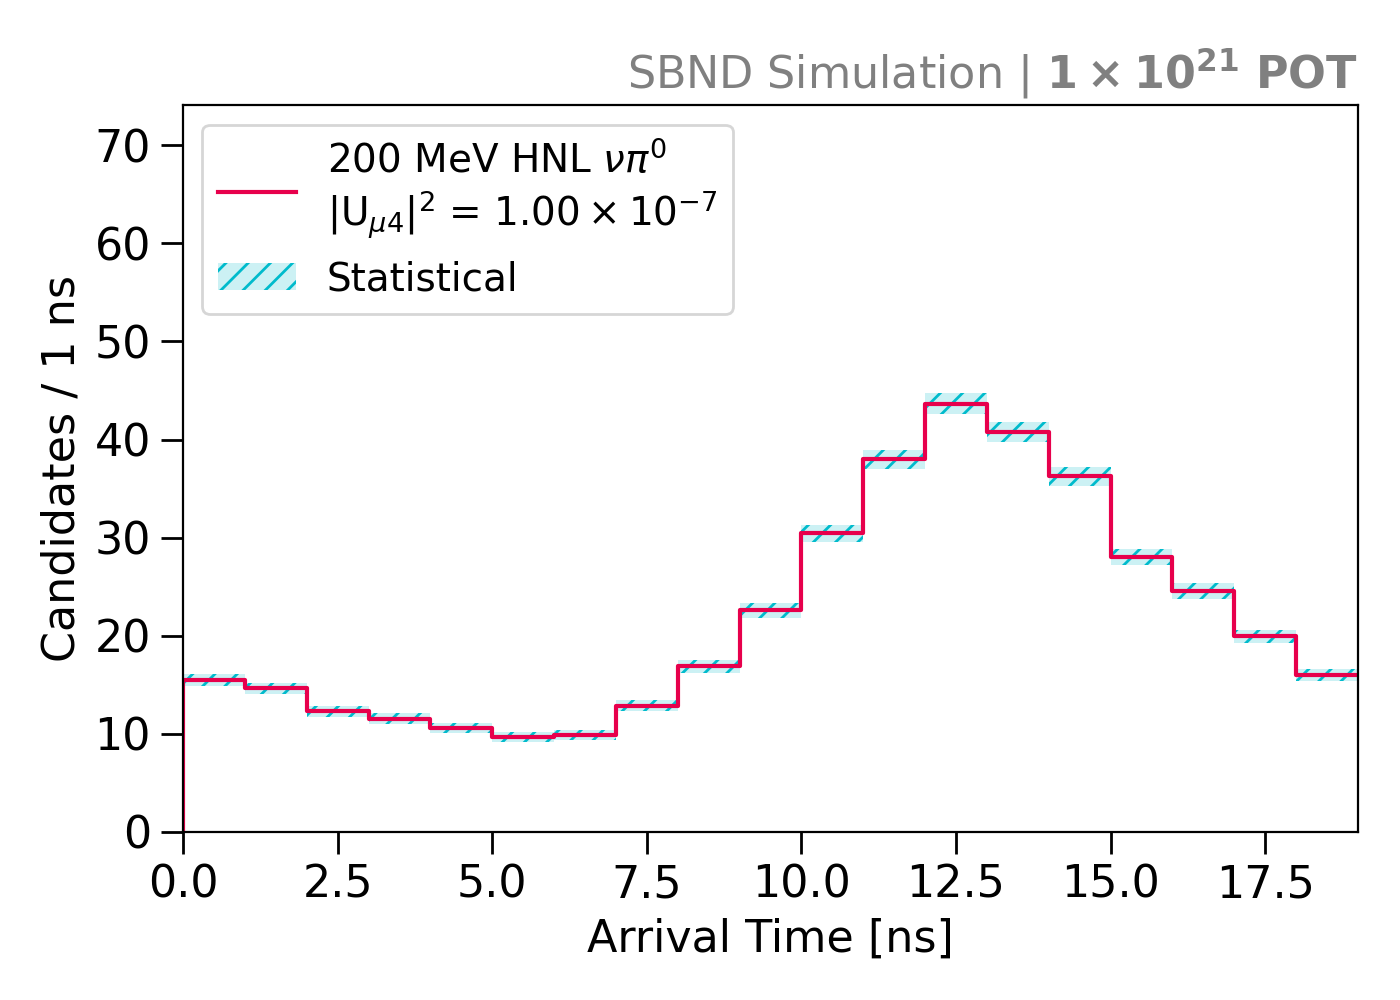
\includegraphics[width=\textwidth]{hnl_statistics_error}
            \caption{Statistical}%
            \label{fig:hnl_stat}
        \end{subfigure}
        \hfill
        \begin{subfigure}[b]{0.45\textwidth}   
            \centering 
            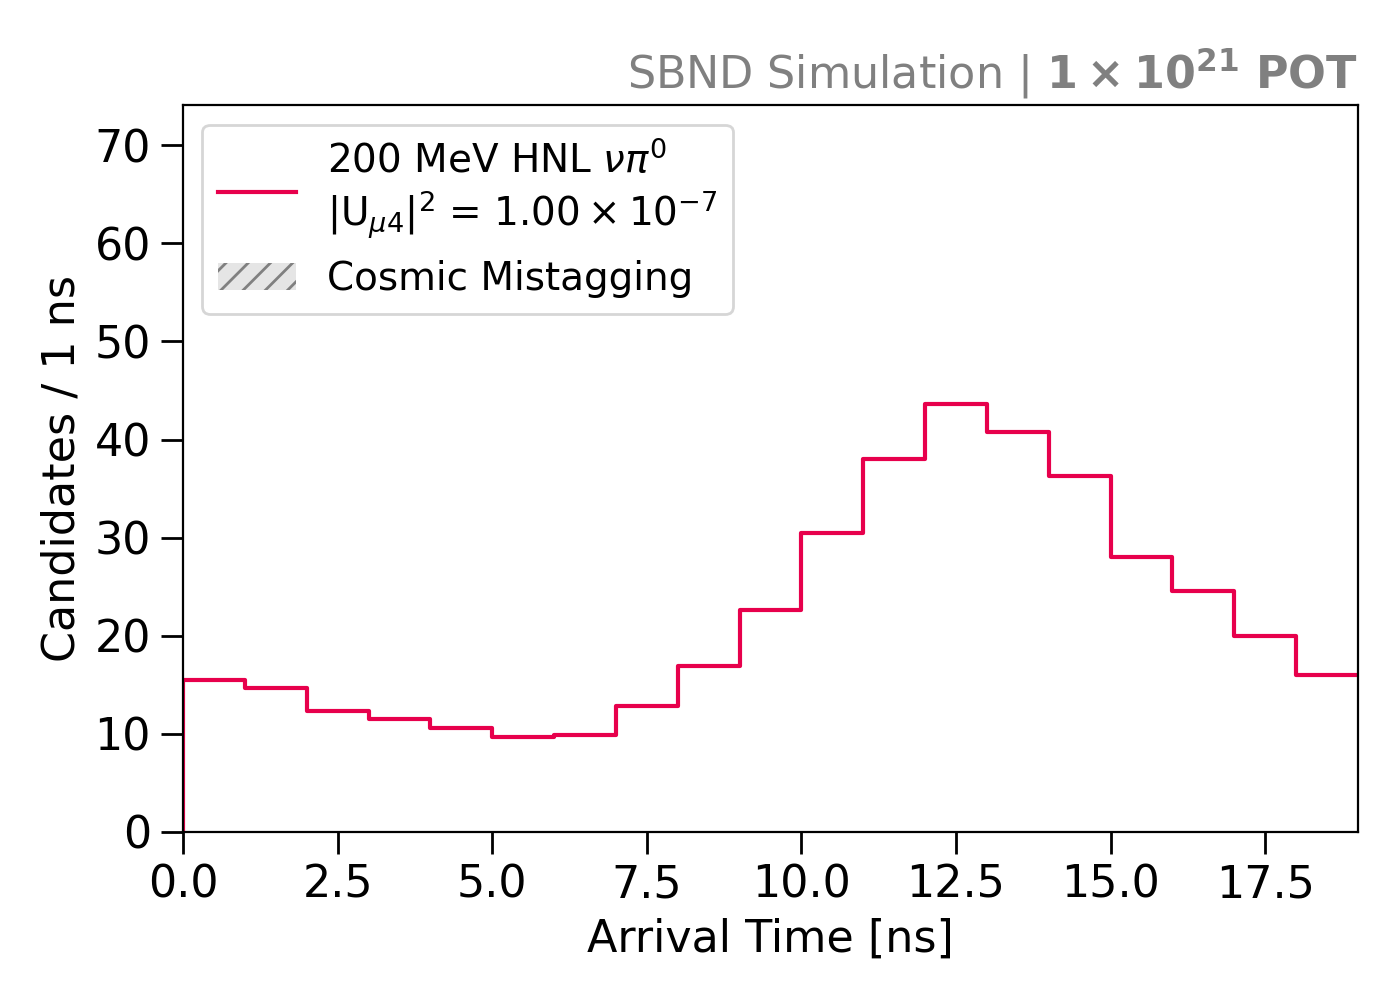
\includegraphics[width=\textwidth]{hnl_mistagging_error}
            \caption{Cosmic Mistagging}%
            \label{fig:hnl_mistag}
        \end{subfigure}
        \centering
        \begin{subfigure}[b]{0.45\textwidth}   
            \centering 
            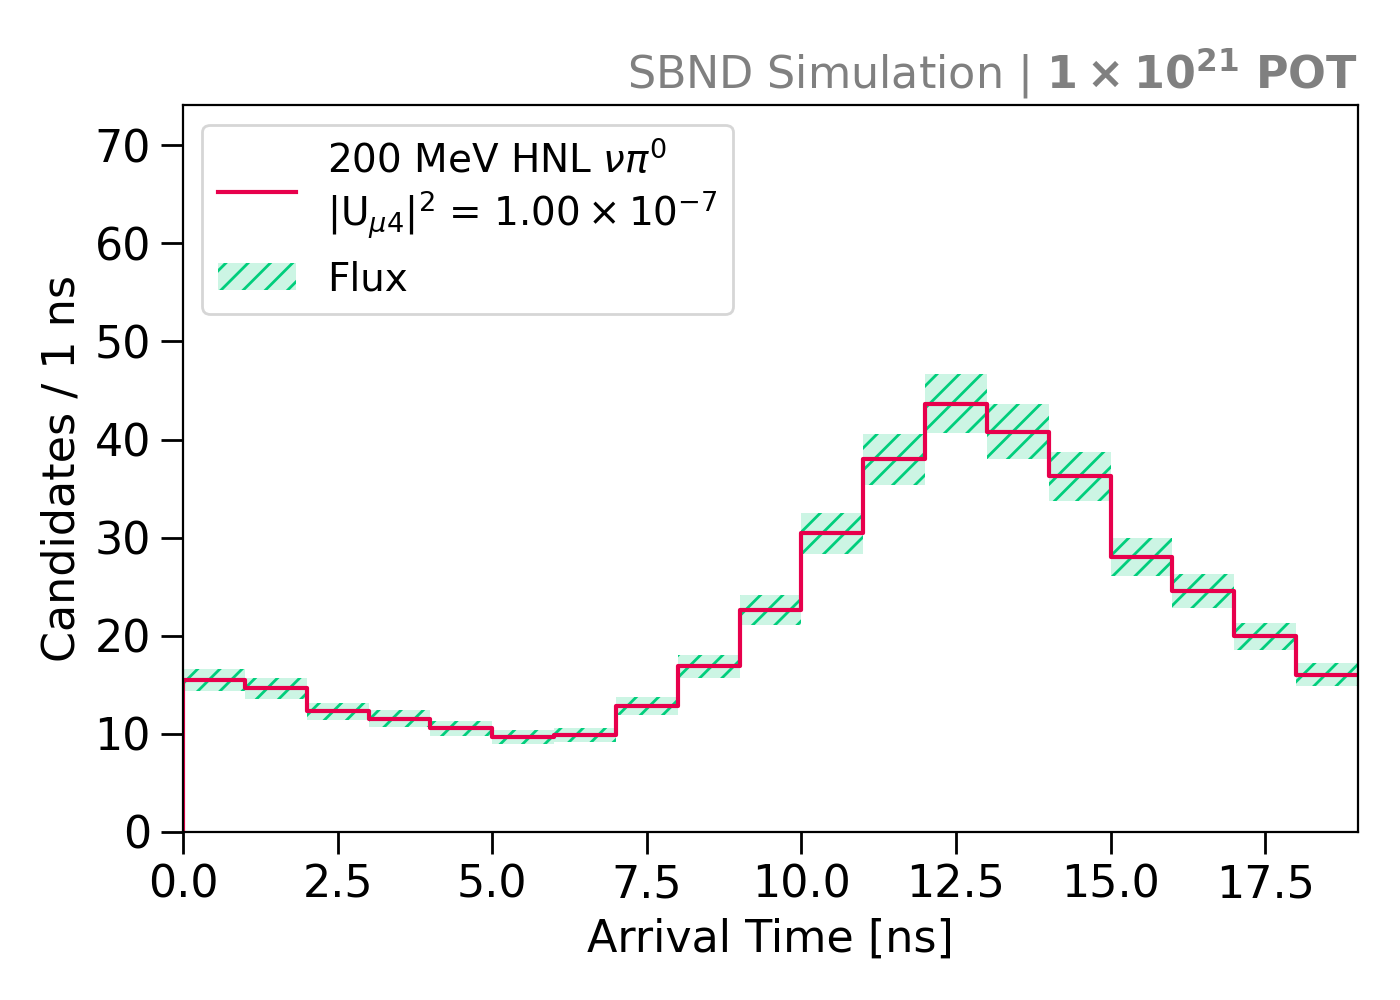
\includegraphics[width=\textwidth]{hnl_flux_error}
            \caption{Flux}%
            \label{fig:hnl_flux}
        \end{subfigure}
	\caption[Uncertainties of Heavy Neutral Leptons]{
		Arrival time distributions of 200 MeV HNLs with (a) statistical, (b) cosmic mistagging and (c) flux uncertainties, normalised to the exposure of $1 \times 10^{21}$ POT and $|U_{\mu4}|^2 = 1 \times 10^{-7}$.
	} 
        \label{fig:hnl_error}
\vspace{0.25cm}
%\end{figure}
%\begin{figure}[htbp!] 
\centering    
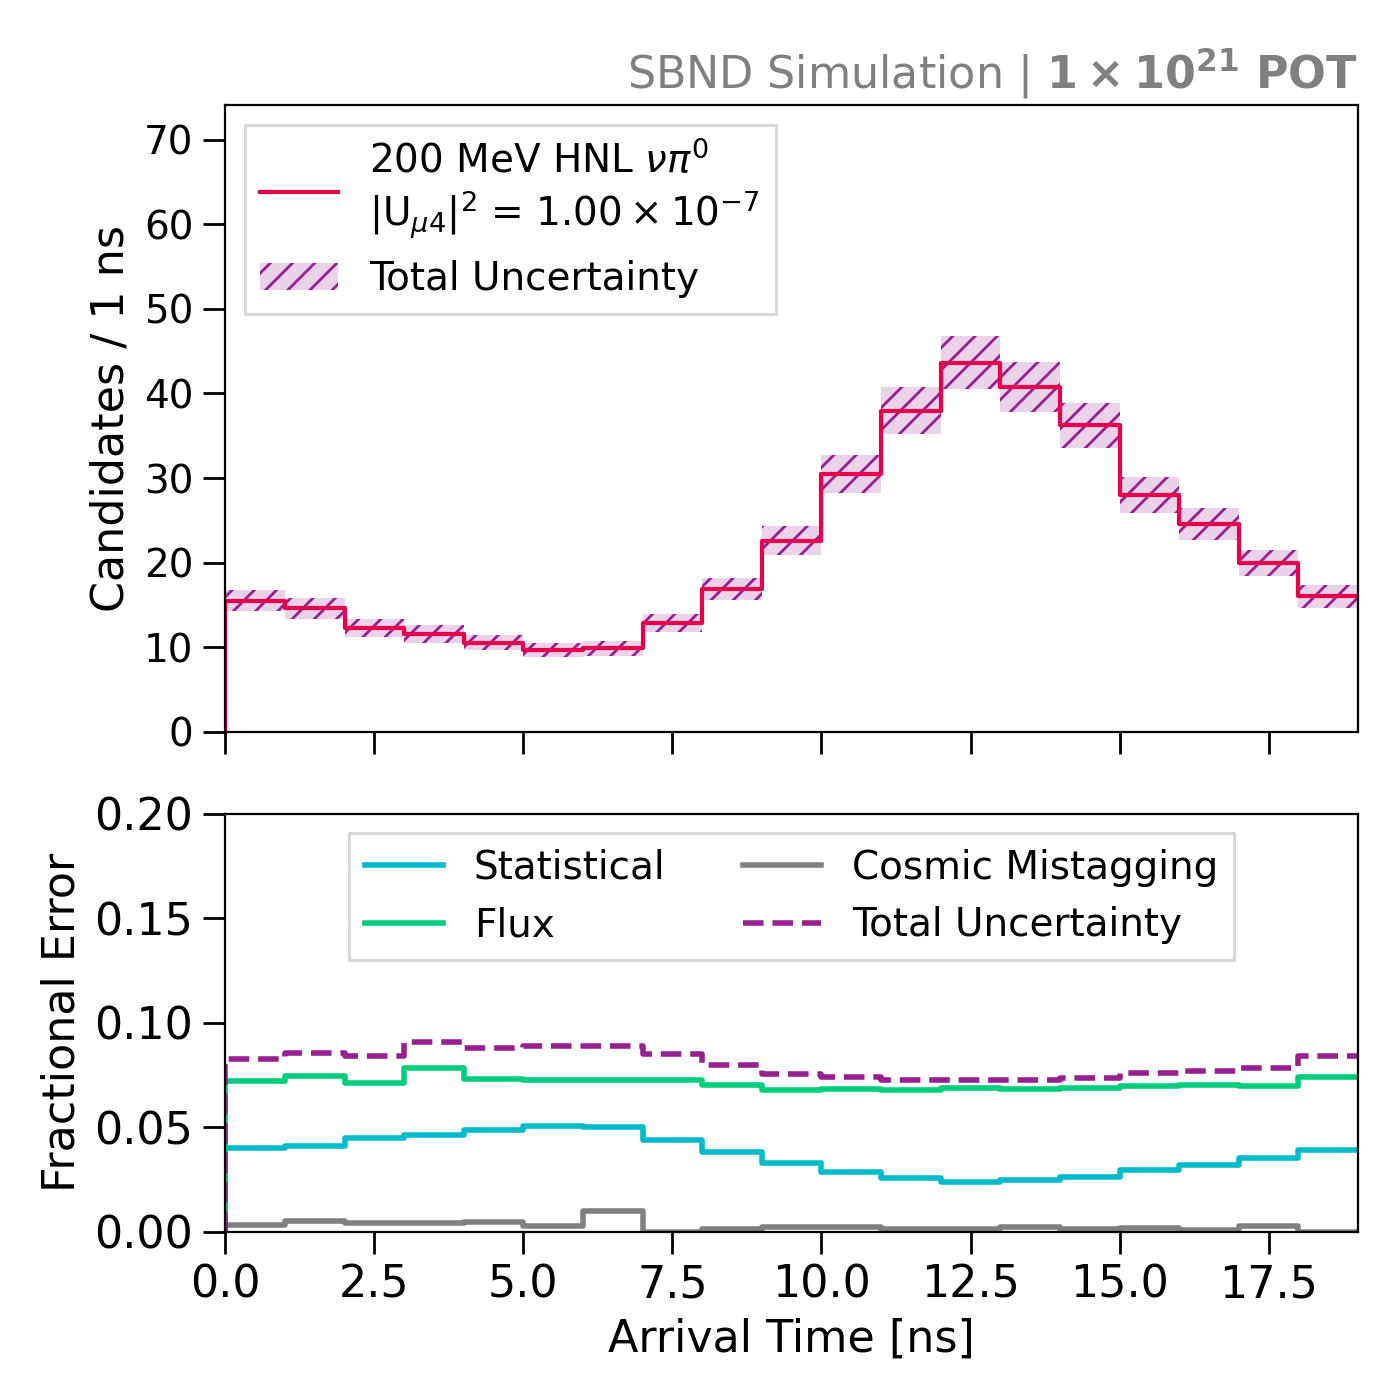
\includegraphics[width=0.5\textwidth]{hnl_error}
\caption[Total Uncertainty and Fractional Uncertainties of Heavy Neutral Leptons]{
Arrival time distribution of 200 MeV HNLs with the total uncertainty (top) and fractional uncertainties (bottom), normalised to the exposure of $1 \times 10^{21}$ POT and $|U_{\mu4}|^2 = 1 \times 10^{-7}$.
}
\label{fig:hnl_total_error}
\end{figure}

The flux systematics was assessed using the reweighting method.
The flux prediction and the reweighting framework for assessing the uncertainties were developed by the MiniBooNE experiment and furthered by the MicroBooNE experiment \cite{BNBFlux, sbnweight_module}.
The framework has been implemented for SBND and intended for a consistent reweighting method across the experiments in the Short-Baseline Neutrino program.
The flux systematics uncertainties as defined in Ref. \cite{BNBFlux} are as follows:
\begin{coloritemize}
	\item \textbf{Proton Delivery}: The proton intensity on the target of the BNB is measured using two toroids, which have an uncertainty of 2\% attributed to calibration.
	\item \textbf{Particle Production}: The flux prediction for the number of secondary mesons produced in the BNB has an uncertainty associated with each particle type (See Section \ref{sec4BNB}). 
		%The model predictions for $\pi^\pm$, $K^\pm$ and $K^0_L$ mesons are previously detailed in Section \ref{sec4BNB}.
		The $K^+$ meson parent of HNLs has the production extrapolated from the global data of $K^+$ using the Feynman Scaling to the relevant BNB energy range, and is constrained by the SciBooNE's direct measurement of $K^+$ from the BNB.
	\item \textbf{Hadronic Interactions}: Hadrons produced in the Be target may interact with Be elastically or inelastically, affecting the kinematics of secondary mesons and consequently, tertiary daughter particles like HNLs and SM neutrinos.
		Cross section uncertainties of $p/n\ +\ $Be and $\pi^\pm\ +\ $Be are propagated through the flux prediction.
	\item \textbf{Horn Magnetic Field}: The magnetic field of the horn impacts the focusing of charged particles produced in the target.
		Uncertainties associated with the horn magnetic field including the current pulsed through the horn and the skin current induced on the surface of the target are computed.
\end{coloritemize}
Fig. \ref{fig:hnl_flux} shows the combined uncertainty of all the flux systematics listed here for HNLs, where the uncertainty is consistent across every bin.
The flux fractional uncertainty is plotted in green in the bottom panel of Fig. \ref{fig:hnl_total_error}, showing that it is constrained $< 8\%$.

Finally, the top figure of Fig. \ref{fig:hnl_total_error} shows the total uncertainty combining the statistical, cosmic mistagging and flux uncertainties.
It can be seen that the total uncertainty is evenly distributed across the arrival time distribution with little biases in any bins. 
The total fractional uncertainty is shown in the purple line in the bottom panel of Fig. \ref{fig:hnl_total_error}, demonstrating that it is well-constrained $< 10\%$ across the entire distribution.


\subsection{Uncertainties of Neutrino and Cosmic Backgrounds}
\label{sec:bkg_error}

For the background of SM neutrinos and cosmic muons, there are four primary sources of uncertainties: (1) statistical, (2) flux, (3) SM neutrino cross section and (4) detector.
The uncertainties due to statistics and flux were computed in the same manner as the uncertainty treatment of the HNL signal.
The detector systematics uncertainty is not included but should be considered in future work.
A new addition is the SM neutrino cross section uncertainty, of which the impact due to the cross section modelling is evaluated using the reweighting method.
Similarly to HNLs, background uncertainties were assessed using the arrival time distribution.  

The statistical uncertainty of the background was computed using using Eq. \ref{eq:stat_err}, taking the number of SM neutrinos and cosmic muons remained after the selection and binned to the arrival time distribution.
Fig. \ref{fig:bkg_stat} shows the statistical uncertainty of the background.
It can be seen that the background statistics are abundant for bins at the centre of the distribution however, limited for bins at the edge.
Therefore, the statistical uncertainty is better constrained for bins at the centre, while bins at the edge have 
a higher statistical fluctuation.
This is also visually evident in the statistical fractional uncertainty plotted in the blue line in the bottom panel of Fig. \ref{fig:bkg_total_error}.
For bins at the centre of the distribution, the statistical fractional uncertainty is constrained at $< 20\%$.
For bins at the edge of the arrival time distribution, particularly the first and last 4 bins, the statistical fractional uncertainty reaches the level about $100\%$.

The flux systematics of the background was measured using the reweighting method similar to HNLs.
One key difference in the flux systematics is that unlike HNLs coming from only $K^+$, SM neutrinos can result from $\pi^\pm$, $K^\pm$ and $K^0_L$.% as previously plotted in Fig. \ref{fig:BNB_neutrino_flux}.
Particularly, the Sanford-Wang parametrisation for modelling the $\pi^+$ production introduces large biases for Neutral Current (NC) $\pi^0$ interactions \cite{EdPhD}, which is the main background contributor.
The resulting flux uncertainty of the background is plotted in Fig. \ref{fig:bkg_flux} and the flux fractional uncertainty is plotted in the green line in the bottom panel of Fig. \ref{fig:bkg_total_error}.
The flux fractional uncertainty is constrained $<20 \%$ and consistent across the entire arrival time distribution.

\begin{figure}[htbp!]
        \begin{subfigure}[b]{0.45\textwidth}   
            \centering 
            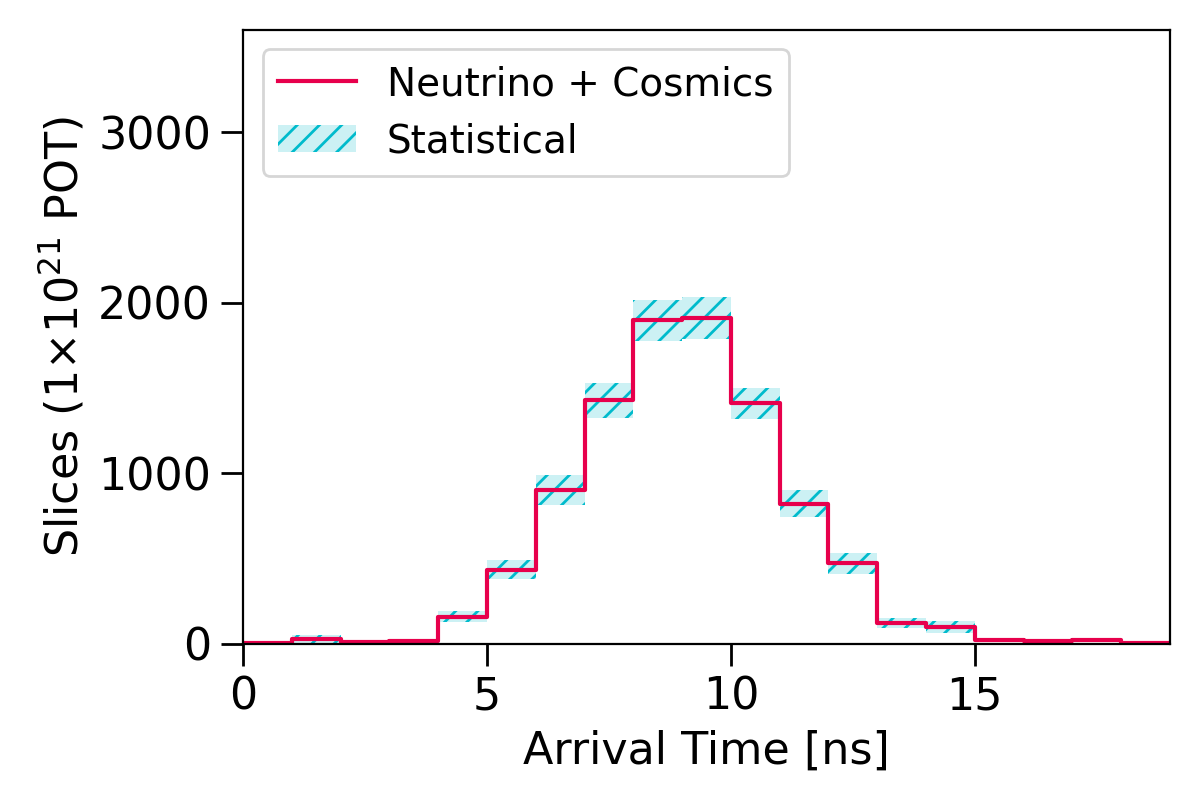
\includegraphics[width=\textwidth]{bkg_statistics_error}
            \caption{Statistical}%
            \label{fig:bkg_stat}
        \end{subfigure}
        \hfill
        \begin{subfigure}[b]{0.45\textwidth}   
            \centering 
            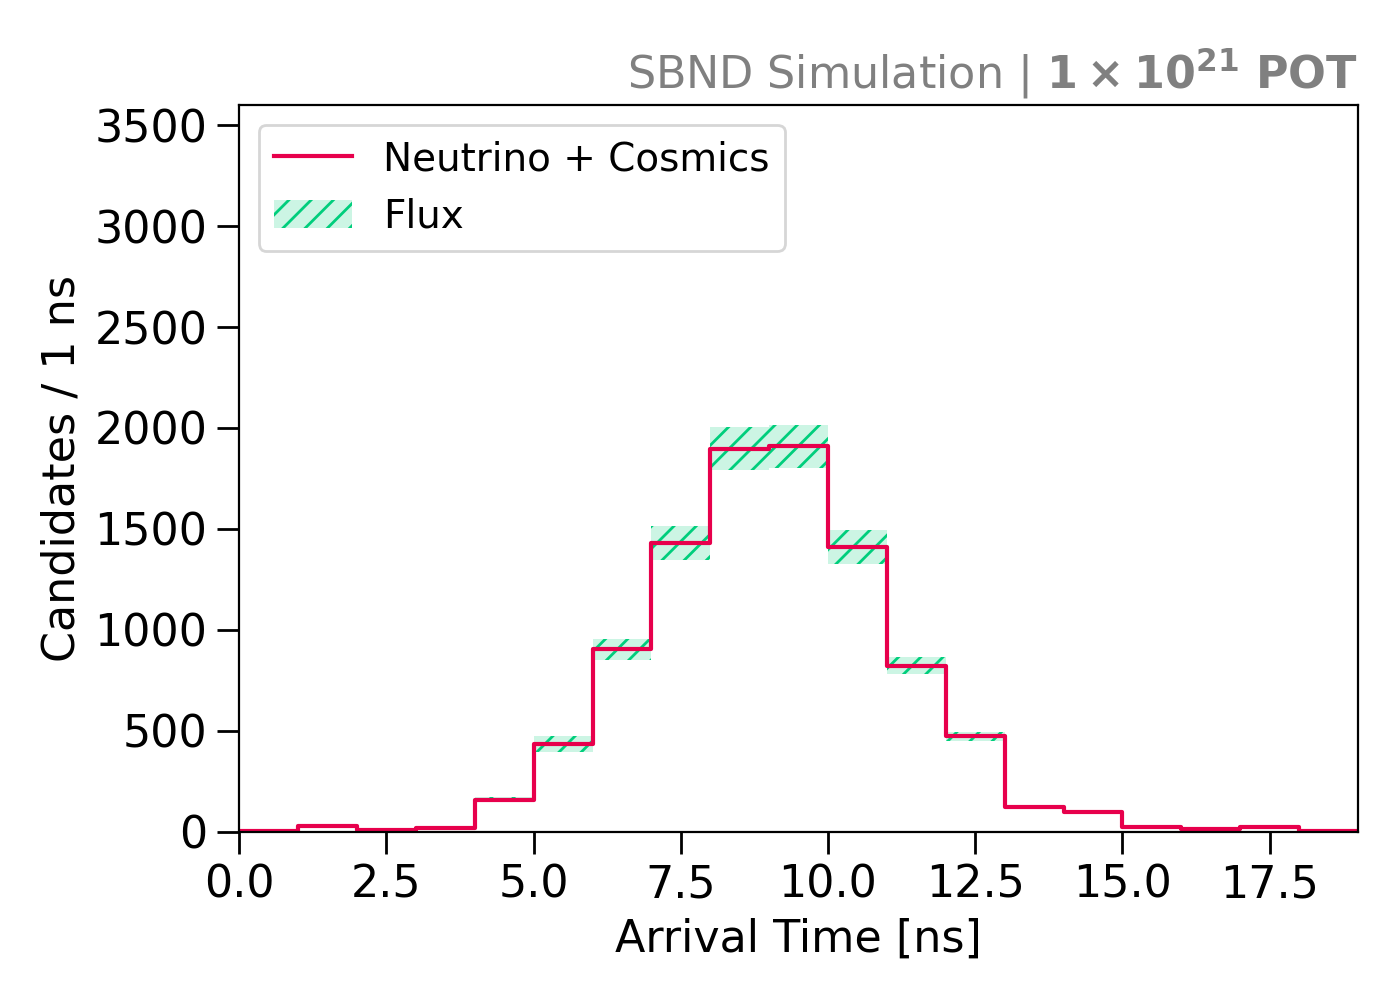
\includegraphics[width=\textwidth]{bkg_flx_error}
            \caption{Flux}%
            \label{fig:bkg_flux}
        \end{subfigure}
        \centering
        \begin{subfigure}[b]{0.45\textwidth}   
            \centering 
            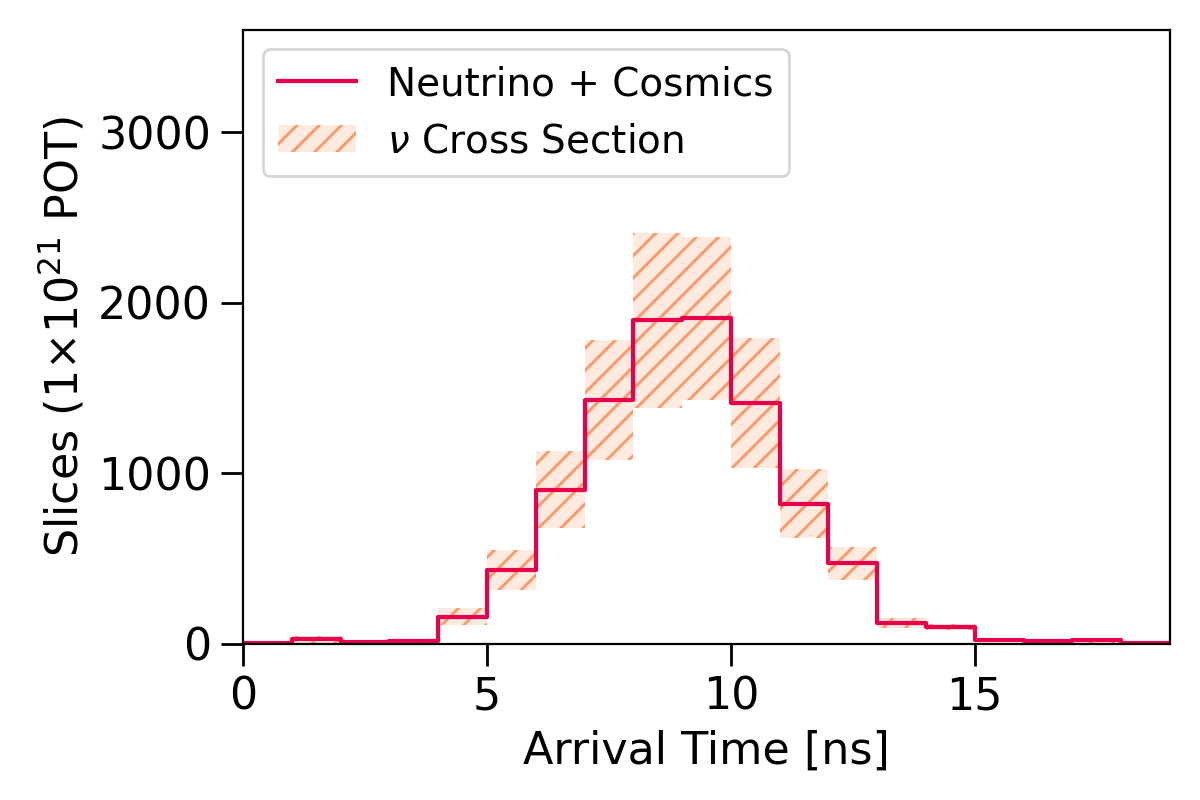
\includegraphics[width=\textwidth]{bkg_xsec_error}
            \caption{SM Neutrino Cross Section}%
            \label{fig:bkg_xsec}
        \end{subfigure}
	\caption[Uncertainties of SM Neutrinos and Cosmic Backgrounds]{
		Arrival time distributions of SM neutrino and cosmic backgrounds with (a) statistical, (b) flux and (c) SM neutrino cross section uncertainties, normalised to the exposure of $1 \times 10^{21}$ POT.
	}
        \label{fig:bkg_error}
\vspace{0.15cm}
%\end{figure}
%\begin{figure}[htbp!] 
\centering    
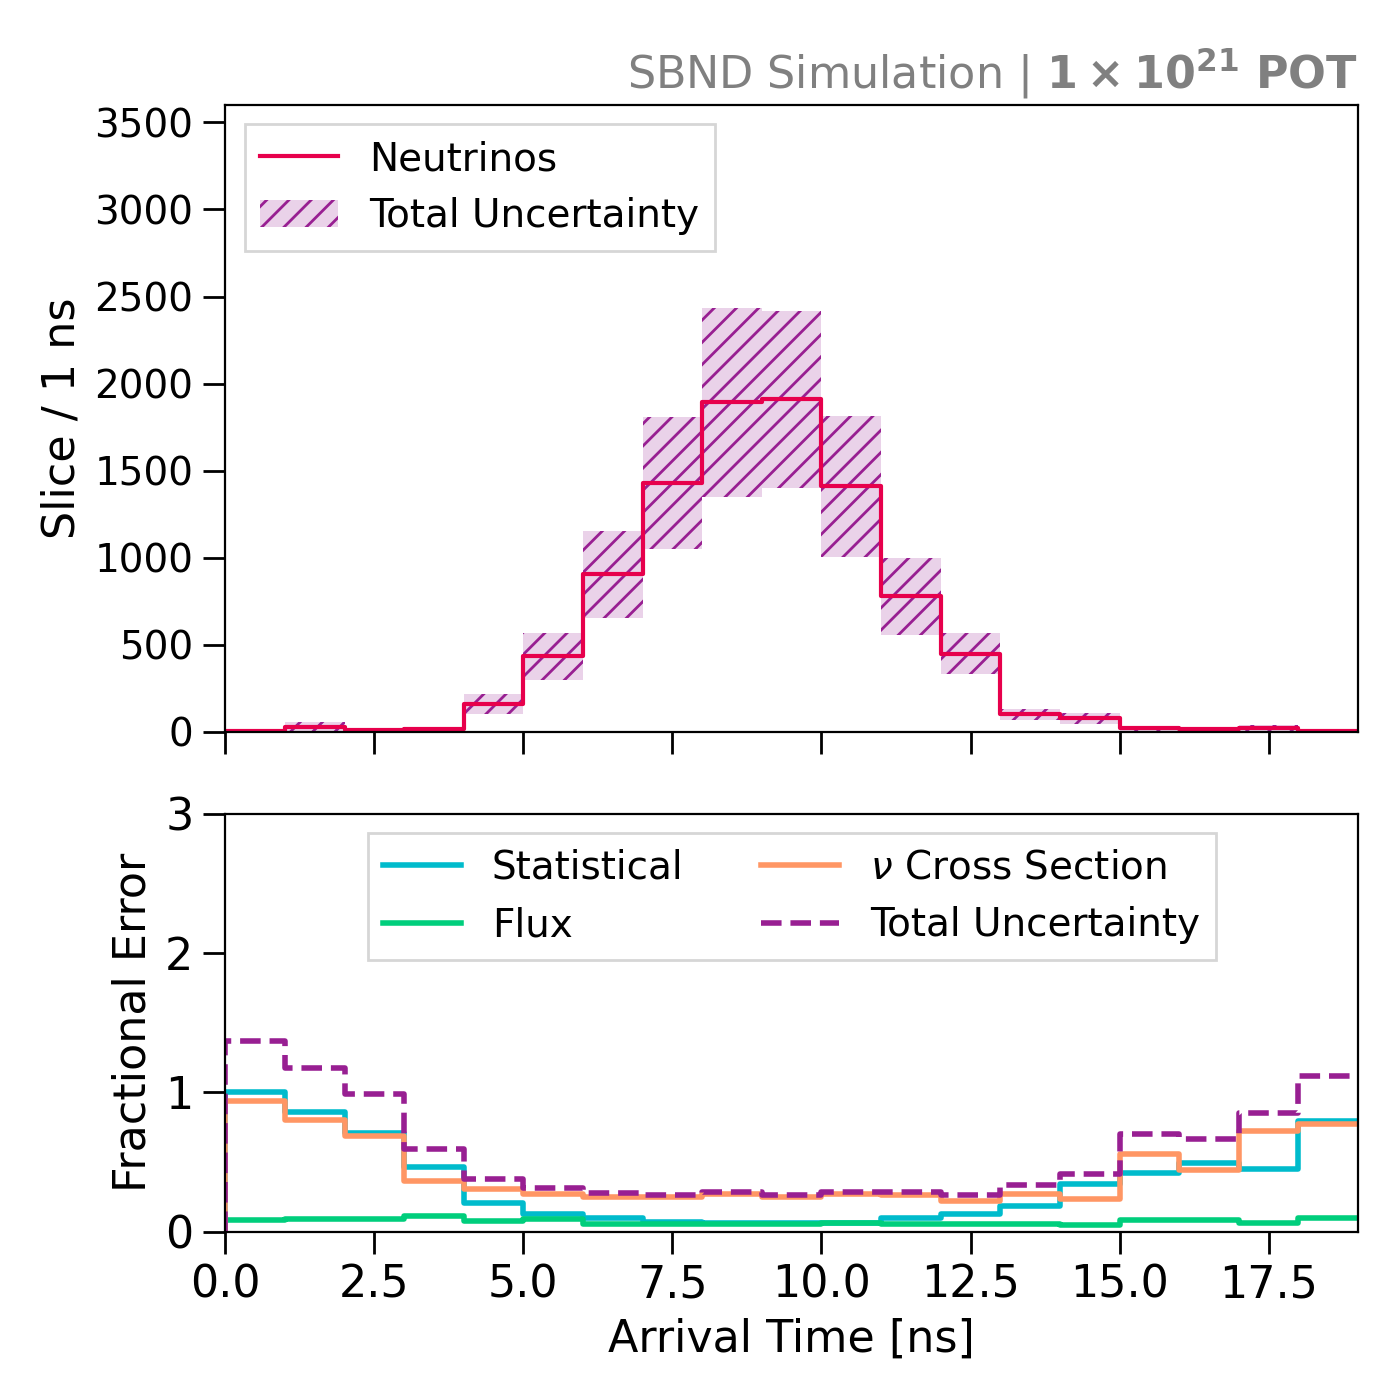
\includegraphics[width=0.5\textwidth]{bkg_error}
\caption[Total Uncertainty and Fractional Uncertainties of SM Neutrinos and Cosmic Backgrounds]{
Arrival time distributions of SM neutrino and cosmic backgrounds with the total uncertainty (top) and fractional uncertainties (bottom), normalised to the exposure of $1 \times 10^{21}$ POT.
}
\label{fig:bkg_total_error}
\end{figure}

%There are two types of weights for SM neutrino interaction cross section: (1) weights associated with a group of correlated physics parameters and (2) weights associated with a single non-correlated physics parameter.
%The SM neutrino systematics for a group of physics parameters are as follows
%\begin{coloritemize}
%\item\textbf{Charged Current Quasi-Elastic Scattering (CC-QE)}: Coefficients of the Z expansion of the axial form factor for CC-QE interactions are varied.
%\item\textbf{Deep Inelastic Scattering (DIS)}: Parameters and correction factors of the Bodek-Yang model, which is used for modelling DIS cross sections, are varied. 
%\item\textbf{Neutral Current Elastic Scattering (NC-EL)}: The axial mass and the strange axial vector of the dipole form factor of NC-EL interactions are varied.
%\item\textbf{Neutral Current Resonant Scattering (NC-RES)}: The axial mass and the strange axial vector of the dipole form factor of NC-RES interactions are varied.
%\item\textbf{Charged Current Resonant Scattering (CC-RES)}: The axial mass and the strange axial vector of the dipole form factor of CC-RES interactions are varied.
%\item\textbf{Hadron Transport Interactions}: The mean free path, inelastic scattering, absorption, and pion production cross section are varied for both pions and nucleons.
%\end{coloritemize}
%The SM neutrino systematics for a single non-correlated physic parameter are as follows
%\begin{coloritemize}
%\item\textbf{Charged Current Quasi-Elastic Scattering (CC-QE)}: The shape of vector form factor, the random phase approximation and the strength of the Coulomb corrections of CC-QE interactions are varied.
%\item\textbf{Meson Exchange Current Interactions (MEC)}: The decay angle and the normalisation factor of CC-MEC and NC-MEC are varied.
%\item\textbf{Coherent Scattering (COH)}: Normalisation factors of NC-COH and CC-COH cross section interactions are varied.
%\item\textbf{NonRES Backgrounds}: Non-resonant backgrounds are varied for CC and NC, $\nu$ and $\bar{\nu}$, neutron and proton, 1$\pi$ and 2$\pi$ for a total of 16 systematics parameters.
%\item\textbf{Angular Distribution}: The angular distribution of $\gamma$ and $\pi$ are varied.
%\item\textbf{Branching Fraction}: The branching fraction scale factor for resonant  decays with either a single $\gamma$ or $\pi$ are varied.
%\end{coloritemize}
The SM neutrino cross section uncertainty was assessed using the reweighting method, with systematics of models employed by the GENIE generator provided in Ref. \cite{genie_tune}.
Fig. \ref{fig:bkg_xsec} shows the resulting combined uncertainty of all the SM neutrino interaction cross section systematics.
Compared to statistical and flux uncertainties, the magnitude of the cross section uncertainty is significantly larger.
This is due to the primary background after selection being NC $\pi^0$, of which the cross section is not well-measured.  
Uncertainties associated with NC cohenrent and NC resonant scattering are the main contributors to this channel.
Moreover, a small fraction of Charged Current (CC) $\nu_e$ interactions remains after selection and the cross section is also not well-measured.
For this channel, uncertainties associated with CC quasi-elastic scattering systematics contribute the most.
Finally, uncertainties for modelling hadron transport interactions are significant contributors to the cross section uncertainty.
%and NonRES backgrounds of NC1$\pi$ interactions 

The cross section fractional uncertainty is plotted in the orange line in the bottom figure of Fig. \ref{fig:bkg_total_error}.
Bins at the centre of the arrival time distribution have the lowest cross section uncertainty in the entire distribution at $< 50\%$.
The uncertainty increases towards the bins at the edge of the distribution, reaching almost $100 \%$ for very low statistics bins.

The total fractional uncertainty combining the statistical, flux and cross section uncertainty, is plotted in purple in the bottom panel of Fig. \ref{fig:bkg_total_error}.
For bins at the edge of the distribution, which are the bins driving the limits, the total uncertainty is particularly high at $> 100\%$ due to the combined contribution from all three uncertainty sources.

%********************************** %First Section  **************************************

\section{Limits Setting Procedure}
\label{sec:limit_procedure}

The sensitivity of SBND to Majorana HNLs is determined as the upper limits on the coupling $|U_{\mu4}|^2$ of HNLs (See Chapter \ref{ChapterHNL}).
The upper limits are set under the assumption of no detected signals so that the results can be directly compared against existing limits in the mass range 140-260 MeV, as previously summarised in Fig. \ref{fig:sensitivity_theory} in Section \ref{sec2Previous}. 
The limits setting procedure employs the likelihood-based hypothesis test \cite{asymptotic_test}, of which likelihood functions are constructed using the arrival time distribution of signals and backgrounds.
The end-to-end procedure was performed using the \texttt{pyhf} package \cite{pyhf_joss}.

The section begins with the hypothesis definitions for upper limits in Section \ref{sec:hypothesis_def} and the construction of the test statistic for each hypothesis in Section \ref{sec:llh_test}.
The CL$_{s}$ method to determine \textit{p}-values of test statistics is described in Section \ref{sec:cls}.
Presented in Section \ref{sec:compute_test} is the computation of test statistics using asymptotic approximation.
Finally, an overview of the limits setting using \texttt{pyhf} is given in Section \ref{sec:set_limits} 

%This section will detail the hypothesis testing .

%Validation of the result acquired from the \textit{pyhf} package and the construction of likelihood functions using \textit{pyhf} are also presented.

%The test statistic is based on the likelihood ratio describing the probability of the observed data under the assumption of model parameters, allowing for the construction of the null and test hypotheses on the parameters.
%The resulting \textit{p}-values from the null and test hypotheses are then used to compute a modified $p$-value using the Confidence Levels (CL$_{s}$) method \cite{CLs_Junk, CLs_Read} to set the upper limits on the coupling $|U_{\mu4}|^{2}$. 

\subsection{Hypothesis Definition}
\label{sec:hypothesis_def}
The setting limit procedure employs the frequentist approach by performing hypothesis testing to quantify the level of agreement between the observed data and a given hypothesis $H$.
To exclude a signal region, the test hypothesis $H_{b}$ is defined as describing only known processes, or a background-only model.
Meanwhile, the null hypothesis $H_{s+b}$ is defined as the model including both background and signal processes.

A given hypothesis $H$ is constructed to represent the expectation value for an observable distribution, which is chosen to be the arrival time distribution.
For a series of observations $n$, the expectation value of the bin $i$ can be constructed as:
\begin{equation}
\label{eq:expectation}
    E[n_i] = \mu s_i + b_i.
\end{equation}
$s_i$ is the number of entries from the HNL signal distribution depicted in Fig. \ref{fig:hnl_total_error} and $b_i$ are the number of entries from the background distribution depicted in Fig. \ref{fig:bkg_total_error}.
The \textit{parameter of interest} $\mu$ determines the strength of the signal process, where $\mu = 0$ corresponds to the background-only $H_{b}$ hypothesis and $\mu = 1$ corresponds to the nominal signal $H_{s+b}$ hypothesis.
%It is an unconstrained parameter and is written separately from other parameters in the hypothesis.
It is written separately from other parameters in the hypothesis.

In the HNL search, varying the parameter $\mu$ is equivalent to varying the coupling $|U_{\mu4}|^{2}$.
%To infer from the signal strength $\mu$ to the coupling $|U_{\mu4}|^{2}$, the proportionality of the number of signals $N_{HNL}$ to the coupling is employed.
The signal rate observed at the detector is proportional to the coupling at the HNL production as well as the coupling at the HNL decay.
The proportionality of the signal strength parameter to the coupling is therefore $\sqrt{\mu} \propto |U_{\mu4}|^{2}$.
For the HNL distribution shown in Fig. \ref{fig:hnl_total_error}, the nominal signals strength $\mu = 1$ corresponds to $|U_{\mu4}|^{2}= 1 \times 10^{-7}$.

Other parameters in the hypothesis represent \textit{nuisance parameters}, denoted as $\theta$.
The null and test hypotheses are formally written as:
\begin{align}
    Null\ hypothesis:\ H_{s+b} = H (\mu = 1, \theta),\\
    Test\ hypothesis:\ H_{b} = H (\mu = 0, \theta).
\end{align}

\subsection{Likelihood-based Test Statistic}
\label{sec:llh_test}

To exclude the null hypothesis $H_{s+b}$ at some Confidence Levels (C.L.), a test statistic is performed for a hypothesised $\mu$ against $H_{s+b}$ and $H_{b}$.
Likelihood-based functions are chosen to construct the test statistic for a multi-binned histogram.
The likelihood function is the product of Poisson probabilities of all bins in the histogram \cite{asymptotic_test}:
\begin{equation}
\label{eq:LLH_func}
    %L(\mu, \boldsymbol{\theta}) =  \prod_{i=1}^{N} \frac{(\mu s_i + b_i)^{n_i}}{n_i!} e^{-(\mu s_i + b_i)}  \prod_{k=1}^{M} \frac{u_k^{m_k}}{m_k!}e^{-u_k}
    L(\mu, \theta) =  \prod_{i=1}^{N} \frac{(\mu s_i + b_i)^{n_i}}{n_i!} e^{-(\mu s_i + b_i)}  \prod_{\theta\in\Theta} c_\theta(a_\theta|\theta).
\end{equation}
The first product describes the likelihood of the distribution $n$ with bin $i$, which is constructed using the arrival time distribution of HNLs as signals and SM neutrinos with cosmics as backgrounds as described in Eq. \ref{eq:expectation}. 
The second product is a function of constrained parameters $\Theta$, containing constraint term $c_\theta(a_\theta|\theta)$ with measurement $a_\theta$ constraining the nuisance parameter $\theta$, 	.
Each uncertainty of signals and backgrounds, as discussed in Section \ref{sec:uncertainty}, corresponds to a constraint term. 

For a hypothesised value of $\mu$, the profile likelihood ratio can be constructed from the likelihood function as \cite{asymptotic_test}:
\begin{equation}
\label{eq:likelihood_ratio}
    \lambda(\mu) = \frac{L(\mu, \hat{\hat{\theta}}(\mu))}{L(\hat{\mu},\hat{\theta})}.
\end{equation}
The numerator is the \textit{conditional} likelihood, where $L$ is maximised for a value $\mu$ being tested and $\hat{\hat{\theta}}(\mu)$ is a function of $\mu$.
The denominator is the \textit{unconditional} maximised likelihood, where $\hat{\mu}$ and $\hat{\theta} = \hat{\hat{\theta}}(\hat{\mu})$ are the best fit parameters to the observed data.

A modification in the likelihood ratio is required for cases where the signal process only increases the mean event rate, such that $\mu \geq 0$.
If the observed data results in the best fit $\hat{\mu} < 0$, then the best level of agreement between the data and the prediction is forced to occur at $\hat{\mu} = 0$.
This is equivalent to the late arrival of HNLs relative to the SM neutrino bucket, which can only increase the event rate for bins on either side of the bucket.
The profile likelihood ratio is modified as \cite{asymptotic_test}:
\begin{equation}
    \Tilde{\lambda}(\mu) =
    \begin{cases}
        \frac{L(\mu, \hat{\hat{\theta}}(\mu) )}{L(0, \hat{\hat{\theta}} (0))}\ \ \ \hat{\mu} < 0, \\
        \frac{L(\mu, \hat{\hat{\theta}}(\mu) )}{L(\hat{\mu}, \hat{\theta})}\ \ \ \hat{\mu} \geq 0, \\
    \end{cases}
\end{equation}
where $\hat{\hat{\theta}} (0)$ is a function of $\mu = 0$. 

From the modified profile likelihood ratio, the test statistic for upper limits is \cite{asymptotic_test}:
\begin{equation}
    \Tilde{q}_\mu = 
    \begin{cases}
        -2\ln\Tilde{\lambda}(\mu)\ \ \ \hat{\mu} \leq \mu 
        \\
        0\ \ \ \ \ \ \ \ \ \ \  \ \ \ \ \hat{\mu} > \mu
    \end{cases}
    = 
    \begin{cases}
        -2\ln\frac{L(\mu, \hat{\hat{\theta}}(\mu) )}{L(0, \hat{\hat{\theta}} (0))}\ \ \ \hat{\mu} < 0, \\
        -2\ln\frac{L(\mu, \hat{\hat{\theta}}(\mu) )}{L(\hat{\mu}, \hat{\theta})}\ \ \ 0 \leq \hat{\mu} \leq \mu, \\
        0\ \ \ \ \ \ \ \ \ \ \ \ \ \ \ \ \ \ \ \ \hat{\mu} > \mu.
    \end{cases}
\end{equation}
In the region $\hat{\mu} > \mu$, equivalent to an upward fluctuation in the data compared to the input models, the test statistic $\Tilde{q}_\mu$ is set to 0.
For setting an upper limit, this fluctuation does not represent less incompatibility and therefore is not taken into the rejection region of the test.
The resulting value of $\Tilde{q}_\mu$ indicates the level of agreement between the observed data and the prediction, where a larger value corresponds to an increasing disagreement.

The distribution $f(\Tilde{q}_{\mu}|\mu^{\prime})$ of a test statistic $\Tilde{q}_\mu$ can be interpreted as a PDF.
The subscript of $\Tilde{q}$ refers to the value of $\mu$ being tested in the numerator of the likelihood ratio in Eq. \ref{eq:likelihood_ratio}. 
The second argument $\mu^{\prime}$ refers to the value of $\mu$ being assumed in the denominator of Eq. \ref{eq:likelihood_ratio}.
%As previously defined, $\mu^\prime = \hat{\mu}$ is the value that best describes the observed data.
For setting an upper limit with hypotheses testing, the PDF of interest is $\Tilde{q}_{\mu}$ under the assumption of a different strength parameter $\mu^{\prime} \neq \mu$.
Therefore, the corresponding PDFs for a test signal strength $\mu$, under the assumption of the null hypothesis $H_{s+b}$ and the test hypothesis $H_b$, are respectively as:
\begin{align}
    f(\Tilde{q}_\mu | s + b ) &= f(\Tilde{q}_\mu | \mu^{\prime} = 1 ), \\
    f(\Tilde{q}_\mu | b ) &= f(\Tilde{q}_\mu | \mu^{\prime} = 0 ).
\end{align}

\subsection{The CL$_{\mathrm{s}}$ Method}
\label{sec:cls}

To quantify the level of significance of a test statistic, a $p$-value is computed as an integration of the PDF $f(\Tilde{q}_{\mu}|\mu^{\prime})$ on either side of $\hat{q} = \Tilde{q}_{\mu}(\mu = \hat{\mu}) $, where $\hat{q}$ is the test statistic value from the observed data.
Typically, the $p$-value resulting from a right-sided integration is used to exclude the null hypothesis.
This represents the probability of finding data more background-like assuming that the signal is true.
%, also known as the probability of getting the type I error in hypothesis testing.
%If $p_{s+b} < \alpha$, the null $H_{s+b}$ hypothesis can be excluded with a confidence level of $1 - \alpha$.


%Typically, a right-sided integration represents the probability of finding data of equal or greater incompatibility with prediction under the assumption of $\mu^{\prime}$.

However, this approach does not factor in the probability of finding data under the assumption of the background-only hypothesis.
In scenarios where the test statistic is not sensitive to the prediction models, the PDFs of the $H_{s+b}$ and $H_b$ hypotheses would greatly overlap each other.
One might make the mistake of interpreting having observed data highly contaminated with backgrounds as a statement on the signal hypothesis \cite{CLs_Read}.
The CL$_s$ method addresses this issue by introducing a modified $p$-value, to include a penalty accounting for the sensitivity of the test statistic is to the models.
%This statistical method was developed specifically by particle physics experiments for the purpose of discovery as well as exclusion. 
%This is a conservative approximation of the C.L. to account for poor background modelling and/or statistical fluctuations.

The CL$_{s}$ method defines the \textit{p}-values of the hypotheses $H_{s+b}$ and $H_b$ as follows \cite{asymptotic_test, CLs_Junk, CLs_Read}:
\begin{align}
\label{eq:psb}
    p_{s+b} & = \int_{\hat{q}}^{\infty} f(\Tilde{q}_\mu|s+b) d\Tilde{q}_\mu, \\
\label{eq:pb}
    p_{b} & = \int^{\hat{q}}_{-\infty} f(\Tilde{q}_\mu|b) d\Tilde{q}_\mu.
\end{align}
$p_{s+b}$ represents the probability of finding data more background-like under the assumption of the signal+background hypothesis $H_{s+b}$ and $p_b$ represents the probability of finding data more signal-like under the assumption of the background-only hypothesis $H_b$.
The modified \textit{p}-value is computed from the \textit{p}-value for each hypothesis as \cite{asymptotic_test, CLs_Junk, CLs_Read}:
\begin{equation}
\label{eq:cls}
    CL_{s} = \frac{p_{s+b}}{1-p_b}.
\end{equation}
%Since $(1 - p_b)$ only varies between 0 and 1, the resulting CL$_s$ is always greater or equal to $p_{s+b}$.
%Thus, the CL$_{s}$ is more conservative in quantifying the C.L. of hypothesis testing.
The threshold was chosen to be 0.1, such that CL$_{s} < (1 - 0.9)$, equivalent to setting an upper limit with at a C.L. of 90\%.
This level was motivated in order to compare against existing experiment results. 

\subsection{Computing Test Statistic Distributions}
\label{sec:compute_test}

%One way to obtain the PDF of $\Tilde{q}_\mu$ for a given hypothesis is by throwing toys (or pseudo-experiments) sampled from the observables $n$, with constrained nuisance parameters $\theta$. 
%Each toy result represents a potential outcome of $\Tilde{q}_\mu$ and thus, the toy distribution represent the test statistic $\Tilde{q}_\mu$ distribution.

%Fig, \ref{fig:stat_toy} shows an example PDF of $\Tilde{q}_\mu$ for a test signal strength $\mu$ acquired from 4000 toys thrown.
%The $\Tilde{q}_\mu$ PDF under the assumption of $H_{s+b}$ and $H_b$ is shown in green and yellow respectively.
%The value $\hat{q}_{expected}$ is plotted as the dashed red line.
%The area under the curve $f(\Tilde{q}_\mu | s + b )$ to the right of $\hat{q}_{expected}$ gives the median $p_{s+b}$ and the area under the curve $f(\Tilde{q}_\mu | b )$ to the left gives the median $p_{b}$.
%The CL$_s$ value is then calculated to give the expected limit on the signal strength $\mu$. 
%To identify which $\mu$ value results in CL$_s < 0.1$, a range of $\mu$ is considered until the desired value CL$_s$ is achieved.  
%The test signal strength $\mu$ plotted here gives exactly CL$_s < 0.1$.
%%Variations of 1 and 2 standard deviations from the expected CL$_s$ is then computed.
%\begin{figure}[hp!] 
%\centering    
%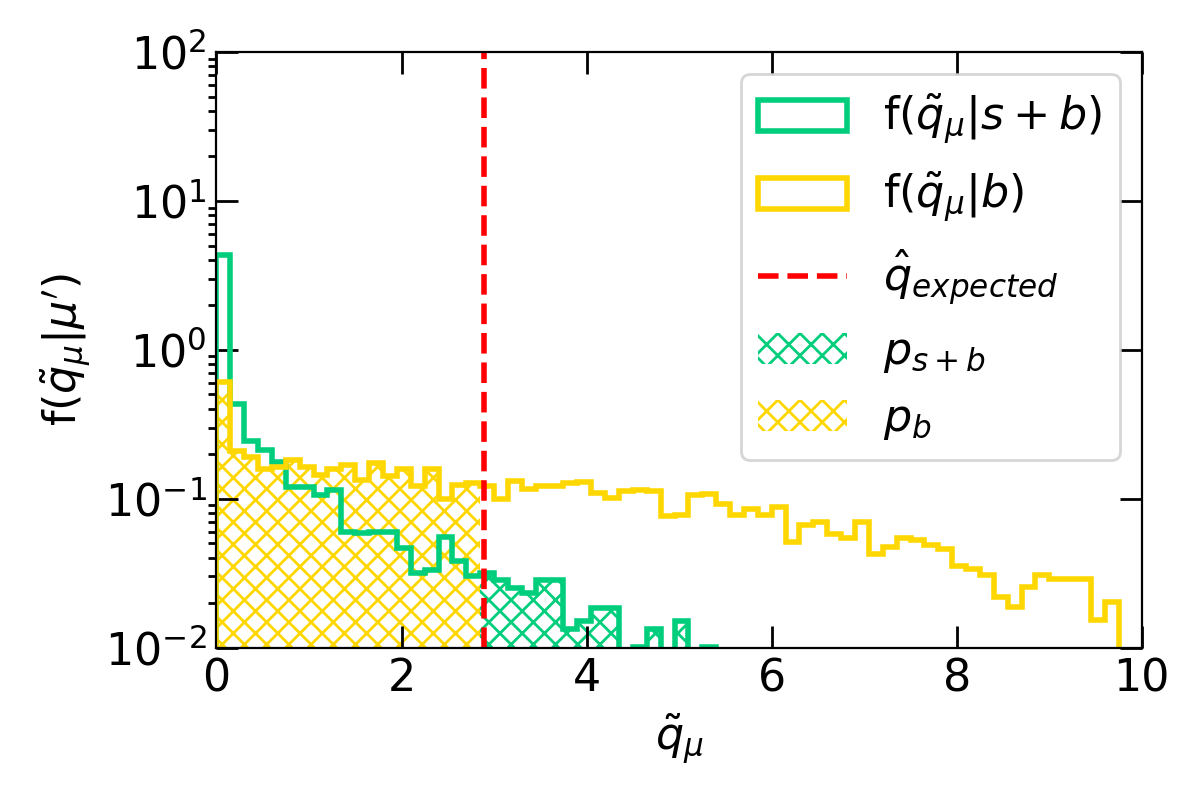
\includegraphics[width=0.65\textwidth]{toy}
%\caption[Distribution of Test Statistics Acquired From Toy Throwing]{Example of $\Tilde{q}_\mu$ distributions using the toy throwing approach.}
%\label{fig:stat_toy}
%\end{figure}
%Similar to the toy throwing approach for an MC study, $\hat{q}_{expected}$ is also taken as the median of the background-only $H_b$ test statistic distribution.

One method to calculate the test statistic $\Tilde{q}_\mu$ and its PDF is by asymptotic approximation.
This approach assumes that $\hat{\mu}$ follows a Gaussian distribution around a mean of $\mu^{\prime}$ with a standard deviation of $\sigma$.
Via the \texttt{pyhf} package, PDFs are computed according to the formulae provided by Ref. \cite{asymptotic_test}.
To determine CL$_s < 0.1$, \texttt{pyhf} scans over a range of $\mu$ and the best value is calculated using interpolation.

\begin{figure}[b!] 
\centering    
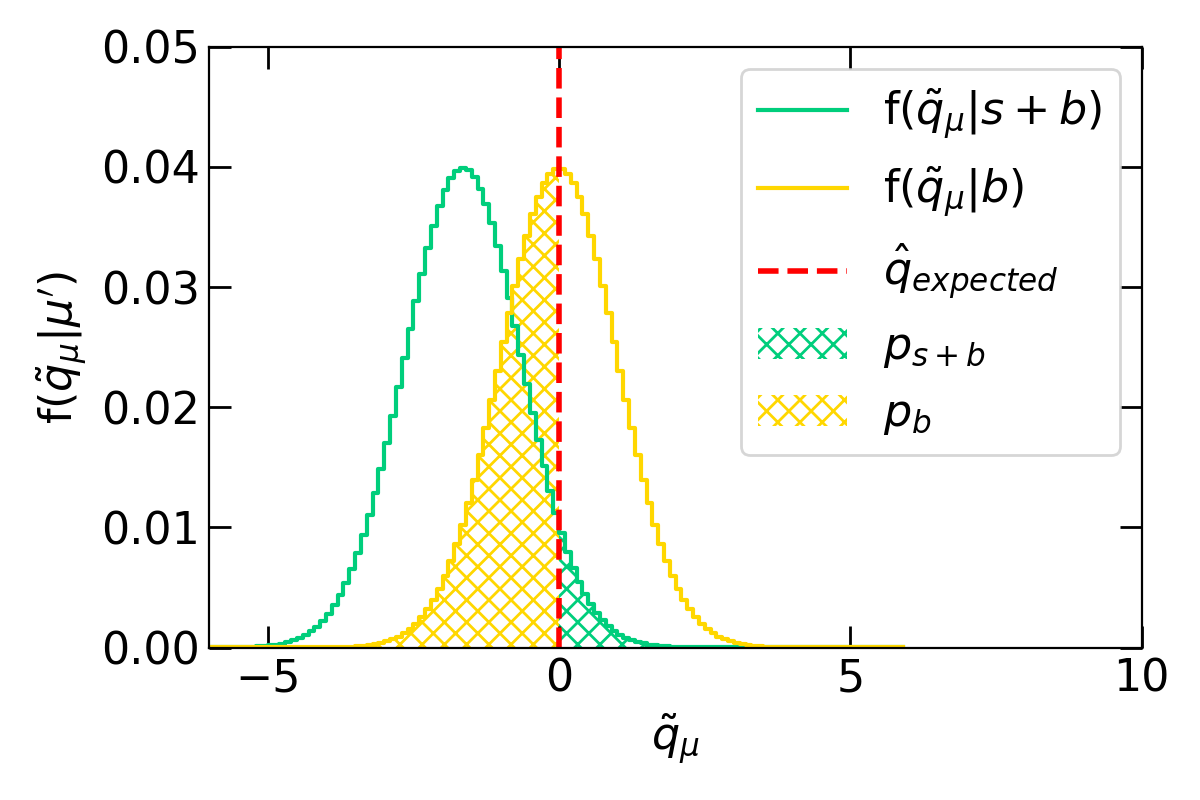
\includegraphics[width=0.55\textwidth]{asymtotic}
\caption[Distribution of Test Statistics Acquired from Asymptotic Approximation]{Example of $\Tilde{q}_\mu$ distributions using the asymptotic approximation.}
\label{fig:stat_asymptotic}
\end{figure}

For a study using MC samples without having the observed data to determine $\hat{q}$, one can consider the distribution under the assumption of the background-only hypothesis $H_b$.
In this case, $\hat{q} = \hat{q}_{expected}$ represents the \textit{expectation} given the model prediction and is taken as the median of the $H_b$ test statistic distribution, equivalent to assuming the observed data is the same as the background-only model. 

Fig. \ref{fig:stat_asymptotic} shows an example PDF of $\Tilde{q}_\mu$ computed using the asymptotic approximation.
The expected $\hat{q}_{expected}$ is plotted as the dashed red line. 
The median $p$-values under the $H_{s+b}$ and $H_b$ hypotheses are plotted as shaded green and yellow areas respectively.
The test signal strength $\mu$ shown here gives CL$_s < 0.1$.
Standard deviations of the CL$_s$ can also be computed by substituting $\mu^\prime$ with $\mu^{\prime} \pm N\sigma$, where $N\sigma$ is the number of standard deviations away from the mean $\mu^{\prime}$. 
%A validation was also carried out to compare the signal strength $\mu$ resulting from the toy throwing and asymptotic approximation.
%Both approaches returned $\mu$ values within 5\% of each other, showing a good agreement.

\subsection{Setting the Upper Limits}
\label{sec:set_limits}

The setting limit procedure was performed fully using the \texttt{pyhf} package, with the test statistic described in the previous section.
The arrival time distributions were input into the \texttt{pyhf} package to infer the upper limit at a C.L. of 90\%.
The distributions input to the background-only $H_{b}$ and the signal+background $H_{s+b}$ hypotheses are as following:
\begin{itemize}
    \item $H_b$: The SM neutrinos and cosmic arrival time distribution.
    \item $H_{s+b}$: The HNL arrival time distribution on top of the background distribution. 
\end{itemize}

These distributions are the ingredients for the first product in Eq. \ref{eq:LLH_func}.
Since the likelihood functions are products of individual bins of the distributions, one can reduce the computing time by considering only high signal-to-noise bins that contribute the most to the limits. 
As previously stated as the timing cut (See Section \ref{sec:select_result}), the relevant high signal-to-noise bins are the first and last 4 bins of the arrival time distribution, which lead to the same result to be demonstrated later.

Three arrival time distributions were used in the limits setting.
Appendix \ref{appendix_lenient} and \ref{appendix_stringent} contain the arrival time distributions for signals and backgrounds after the lenient and stringent cut respectively (See Section \ref{sec:select_result}), with all uncertainties propagated (See Section \ref{sec:uncertainty}) . 
Additionally, Appendix \ref{appendix_smeared} contains the smeared true distributions under the assumption of a timing reconstruction improvement (See Section \ref{sec:truth_bucket}).
%, also used in the same limits setting.

The uncertainties of the arrival time distribution discussed in Section \ref{sec:uncertainty} are the constraints on the nuisance parameters $c_\theta(a_\theta|\theta)$ in the second product Eq. \ref{eq:LLH_func}.
Different types of constraints can take different statistical shapes, which are called \textit{modifiers} in the \texttt{pyhf} package \cite{pyhf_joss}.
Table \ref{table:constraint} summarises the uncertainties and their corresponding modifiers of the signal and background distribution.

For the HNL signal distribution, the assumption is that the signal rate is relatively low and expected to follow a Poisson distribution.
Similarly, the cosmic mistagging rate falls under the same assumption since it is proportional to the signal rate. 
Thus, the modifier for both statistical and cosmic mistagging uncertainties of the signal distribution follows a Poisson shape, treating each bin uncorrelated. 
The flux uncertainty of the signal distribution uses a Gaussian-shaped modifier instead, to enable correlation bin-wise.

For the background distribution, the treatment of statistical uncertainty employs a modified version of the Beeston-Barlow method \cite{BeestonBarlow} to account for statistical fluctuations due to finite statistics.
The modifier in this case follows a Gaussian shape for bins with high statistics and falls back to a Poisson shape for bins with low statistics while treating each bin uncorrelated.
Moreover, the flux and SM neutrino cross section uncertainty also use a Gaussian-shaped modifier, however, with correlation bin-by-bin.

\begin{table}[htbp!]
\caption[Summary of Uncertainty Constraints]{Summary of modifiers used to constrain uncertainties.}
\label{table:constraint}
\begin{center}
\begin{tabular}{|c| c | c | c | c |} 
\hline 
& \textbf{Uncertainty} & \textbf{Modifier} & \textbf{Sample Correlation} & \textbf{Bin Correlation}\\
\hline &&&&\\[-1.5ex]

\multirow{3}{*}{\rotatebox[origin=c]{90}{\parbox[c]{1.85cm}{\centering \textbf{Signal} }}} 

& Statistical & \multicolumn{1}{c|}{Poisson} & \multicolumn{1}{c|}{False} & \multicolumn{1}{c|}{False} \\ [1ex]

& Cosmic mis-tagging & \multicolumn{1}{c|}{Poisson} & \multicolumn{1}{c|}{False} & \multicolumn{1}{c|}{False} \\ [1ex]

& Flux & \multicolumn{1}{c|}{Gaussian} & \multicolumn{1}{c|}{False} & \multicolumn{1}{c|}{True} \\ [1ex]

\hline &&&&\\[-0.5ex]

\multirow{3}{*}{\rotatebox[origin=c]{90}{\parbox[c]{1.95cm}{\centering \textbf{Background} }}} 

& Statistical & \multicolumn{1}{c|}{Gaussian} & \multicolumn{1}{c|}{False} & \multicolumn{1}{c|}{False} \\ [1ex]

& Flux & \multicolumn{1}{c|}{Gaussian} & \multicolumn{1}{c|}{False} & \multicolumn{1}{c|}{True} \\ [1ex]

& SM Neutrino Cross Section & \multicolumn{1}{c|}{Gaussian} & \multicolumn{1}{c|}{False} & \multicolumn{1}{c|}{True} \\ [1ex]
\hline
\end{tabular}
\end{center}
\end{table}

For a single mass point, \texttt{pyhf} performs a scanning of signal strength $\mu$ until the desired $\mu$ value giving the 90\% C.L. is determined. 
To infer from the signal strength $\mu$ to the coupling $|U_{\mu4}|^{2}$, the proportionality $\sqrt{\mu} \propto |U_{\mu4}|^{2}$ is employed.
%The signal rate observed at the detector is proportional to the coupling at the HNL production as well as the coupling at the HNL decay, and thus, $N_{HNL} \propto |U_{\mu4}|^{4}$.
%The upper limit of the coupling is then $\sqrt{\mu}$ multiplied by the input coupling $|U_{\mu4}|^{2}$.
This process was repeated for all HNL masses to acquire the limit contour between 140 and 260 MeV.
%********************************** %First Section  **************************************

\section{Results}
\label{sec:result}

Upper limits from three different arrival time distributions are presented in this section.
The first two distributions were acquired by using fully reconstructed MC samples mimicking data, of which one was applied with a lenient selection as shown in Fig. \ref{fig:final_relaxed} and the other one was applied with a stringent selection as shown in Fig. \ref{fig:final_strict}.
The third distribution is the smeared true as shown in Fig. \ref{fig:final_truth}, which was acquired by smearing \textit{true} variables without any detection simulation and reconstruction applied.
\begin{figure}[htbp!]
        \begin{subfigure}[b]{1.0\textwidth}
            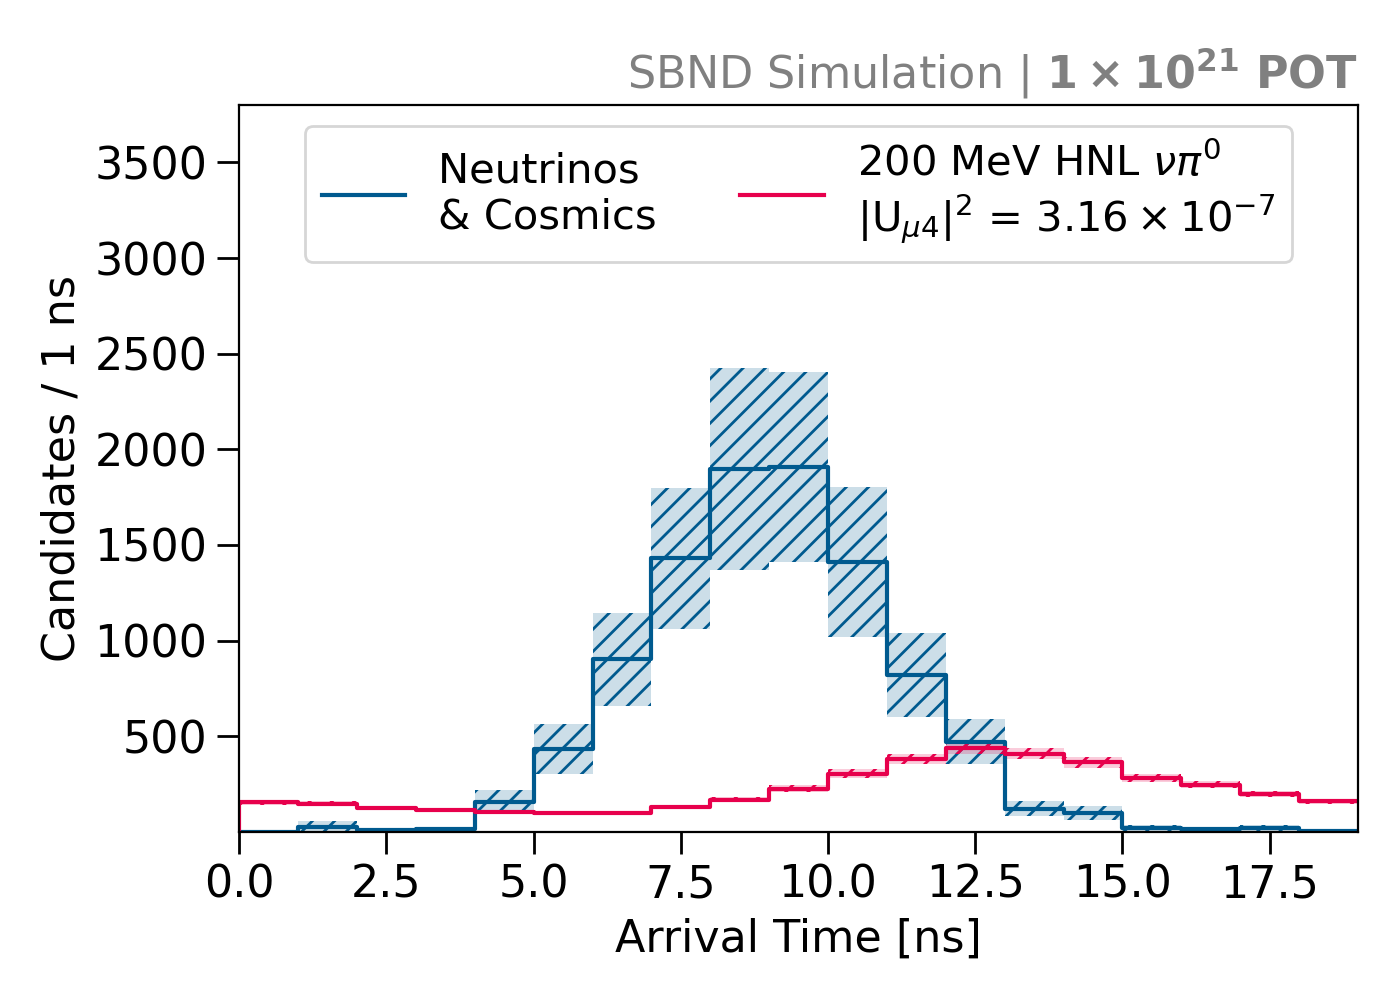
\includegraphics[width=0.5\textwidth]{relaxed_cut}
            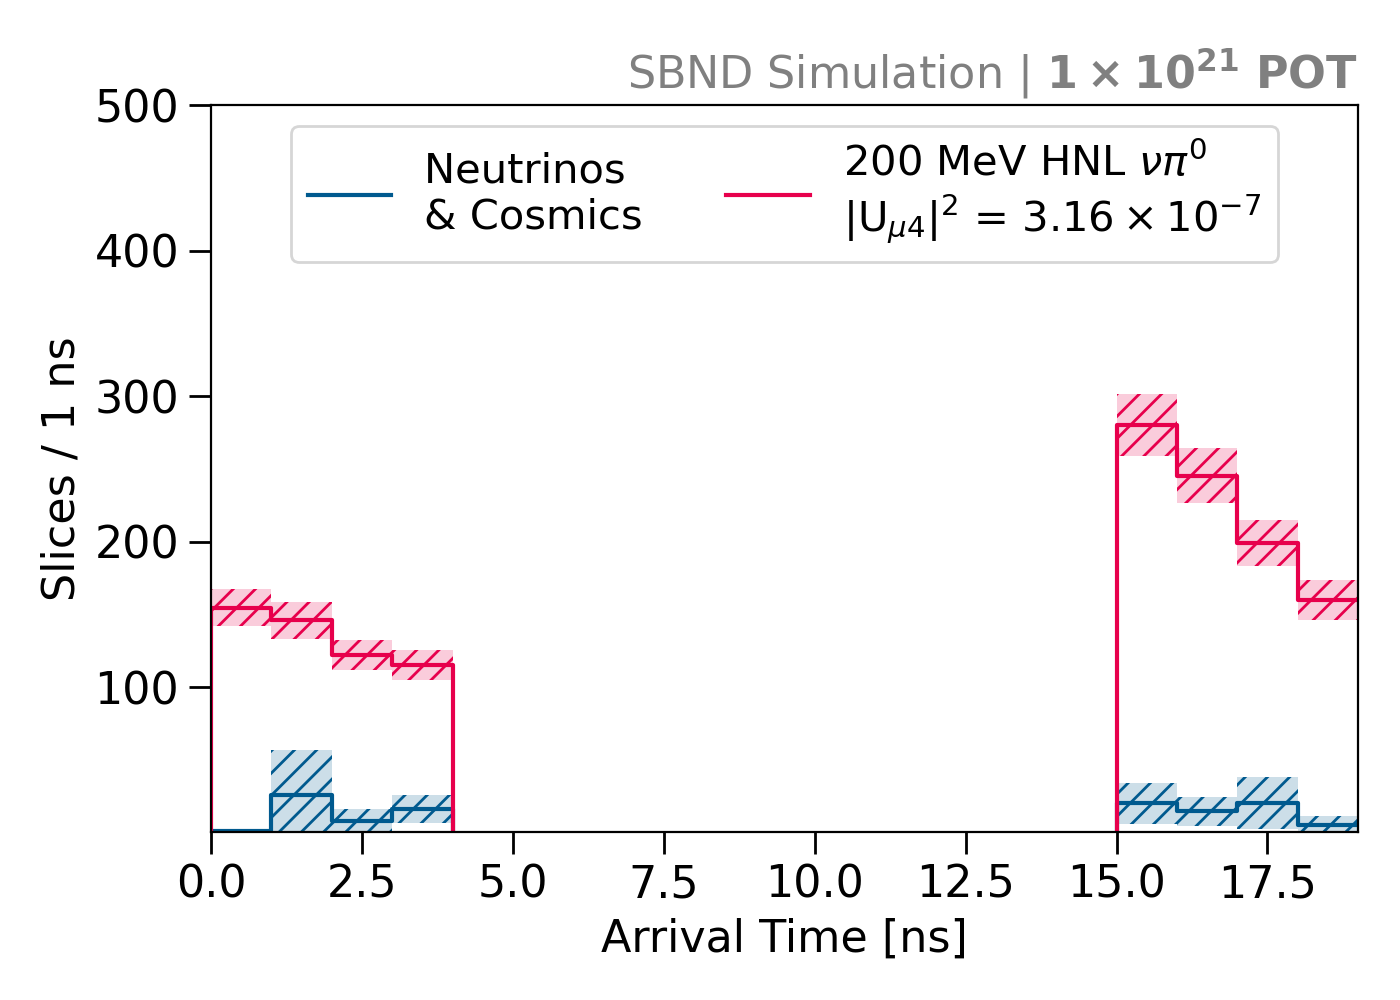
\includegraphics[width=0.5\textwidth]{relaxed_cut_edge}
            \caption{The lenient distribution}%
	    \label{fig:final_relaxed}
     	    \vspace{0.5cm}
        \end{subfigure}
        \begin{subfigure}[b]{1.0\textwidth}
            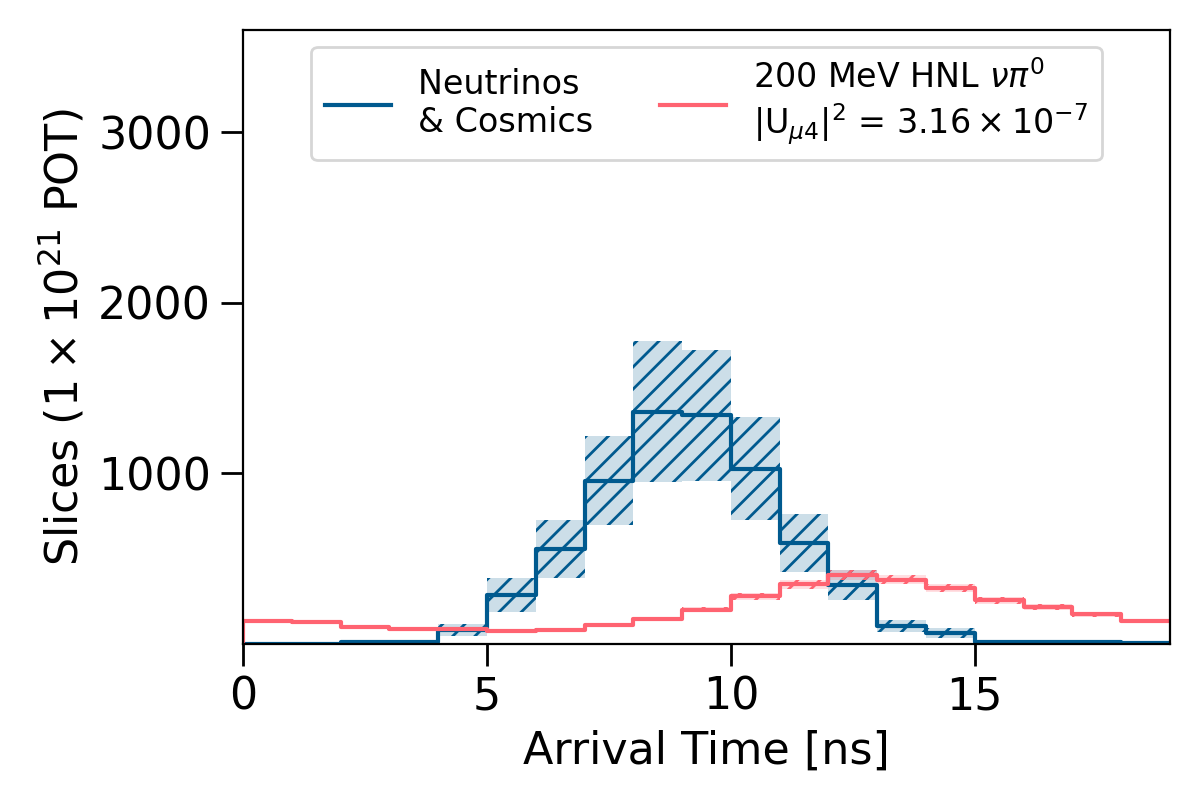
\includegraphics[width=0.5\textwidth]{strict_cut}
            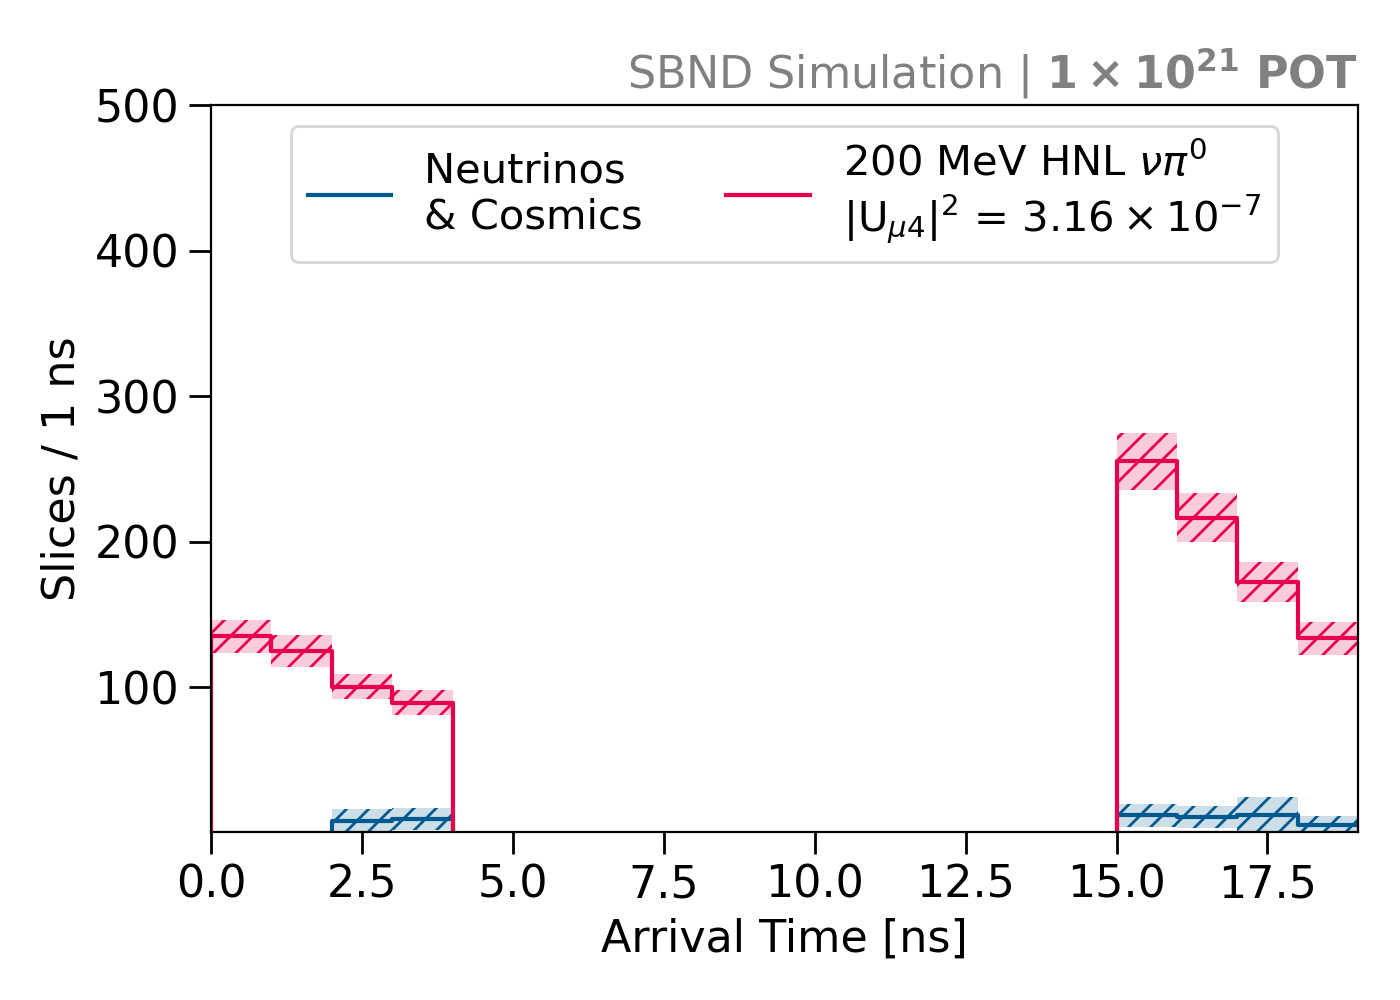
\includegraphics[width=0.5\textwidth]{strict_cut_edge}
            \caption{The stringent distribution}%
	    \label{fig:final_strict}
       	    \vspace{0.5cm}
        \end{subfigure}
        \begin{subfigure}[b]{1.0\textwidth}
            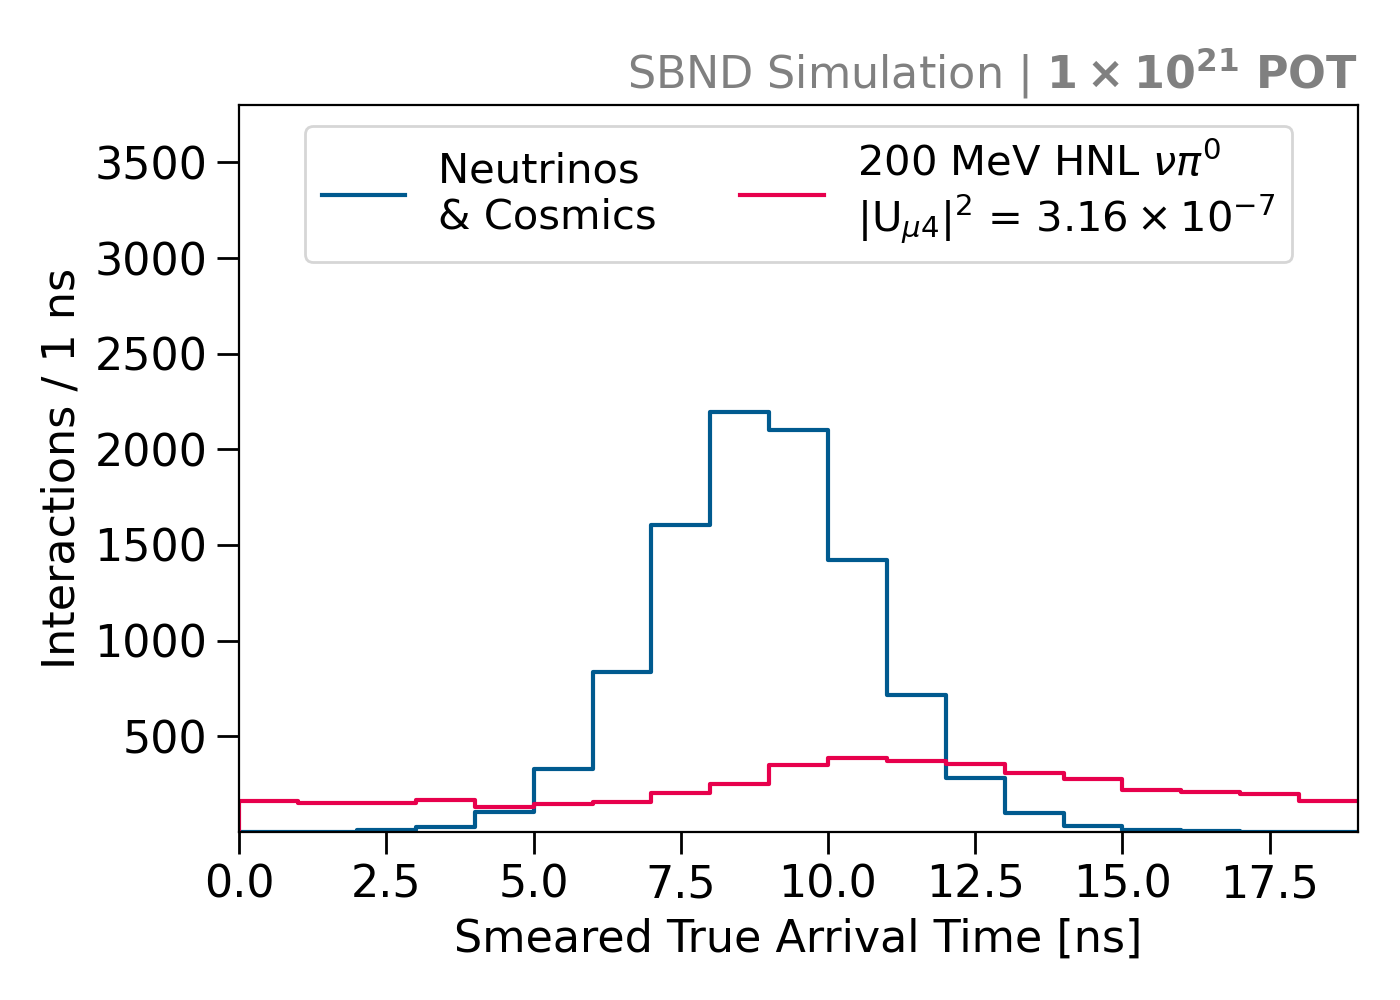
\includegraphics[width=0.5\textwidth]{smeared_truth}
            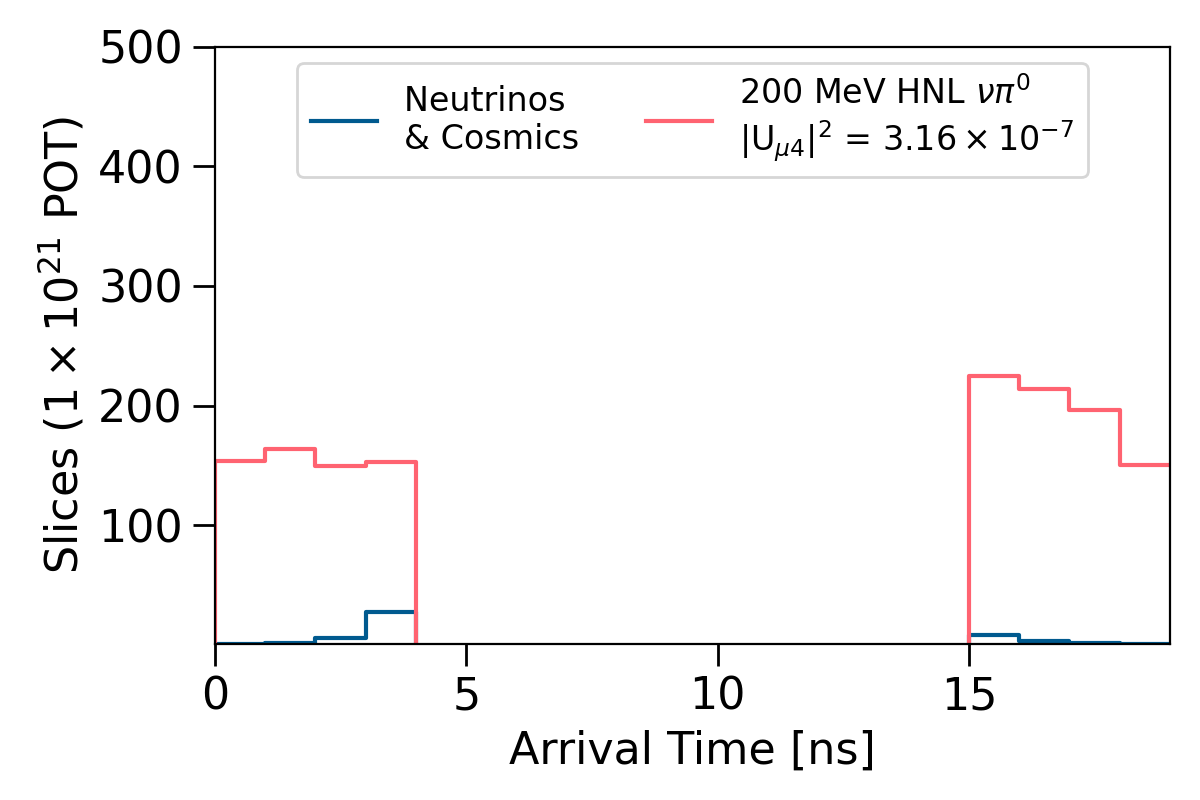
\includegraphics[width=0.5\textwidth]{smeared_truth_edge}
            \caption{The smeared true distribution}%
	    \label{fig:final_truth}
     	    \vspace{0.5cm}
        \end{subfigure}
        \caption[Arrival Time Distributions input to the Limits Setting]{
	Arrival time distributions used in the limits setting, including (a) the lenient, (b) the stringent and (c) the smeared true distribution,
	normalised to the exposure of $1 \times 10^{21}$ POT.
	HNLs of mass 200 MeV is normalised to the coupling $|U_{\mu4}|^2 = 3.16 \times 10{-7}$.
	}
\end{figure}
The smeared true distribution is motivated by a better timing reconstruction to resolve the beam bucket with a resolution of 1.73 ns.
Unlike the reconstructed distributions with uncertainties propagated, the smeared true distribution does not contain any uncertainties for simplicity. 
The first and last 4 bins of every distribution are also shown to demonstrate the exceptionally high signal-to-background ratio of these bins.

\subsection{Comparison Across Different Arrival Time Distributions}

Expected upper limits on the coupling $|U_{\mu4}|^2$ of Majorana HNLs at the 90\% C.L. are presented in Fig. \ref{fig:nupi0_reco_result}, comparing results from the arrival time distribution after the lenient and stringent selection.
The expected limit is plotted as the solid black line.
The deviation band at 1$\sigma$ and 2$\sigma$ away from the expectation, also known as the \textit{Brazil} band, is plotted in shaded green and yellow respectively.
The lenient arrival time distribution results in limits excluding the coupling $|U_{\mu4}|^2$ at the level from $9.18 \times 10^{-7}$ to $1.35 \times 10^{-8}$ across the mass range from 140 to 260 MeV.

On the other hand, the stringent distribution results in more competitive limits, pushing the exclusion region of the coupling further at the level from $5.37 \times 10^{-7}$ to $7.65 \times 10^{-9}$ at the same mass range.
This is due to the stringent distribution having a better signal-to-background ratio for bins at the edge of the distribution.
This is evident when comparing between Fig. \ref{fig:final_relaxed} and \ref{fig:final_strict}, where the signal rate is very similar across the two distributions but the background rate is much lower in the stringent than the lenient distribution.
Particularly, the first two bins of the stringent distribution are background-free, thus, driving the limits significantly.

\begin{figure}[b!]
        \begin{subfigure}[b]{0.495\textwidth}
            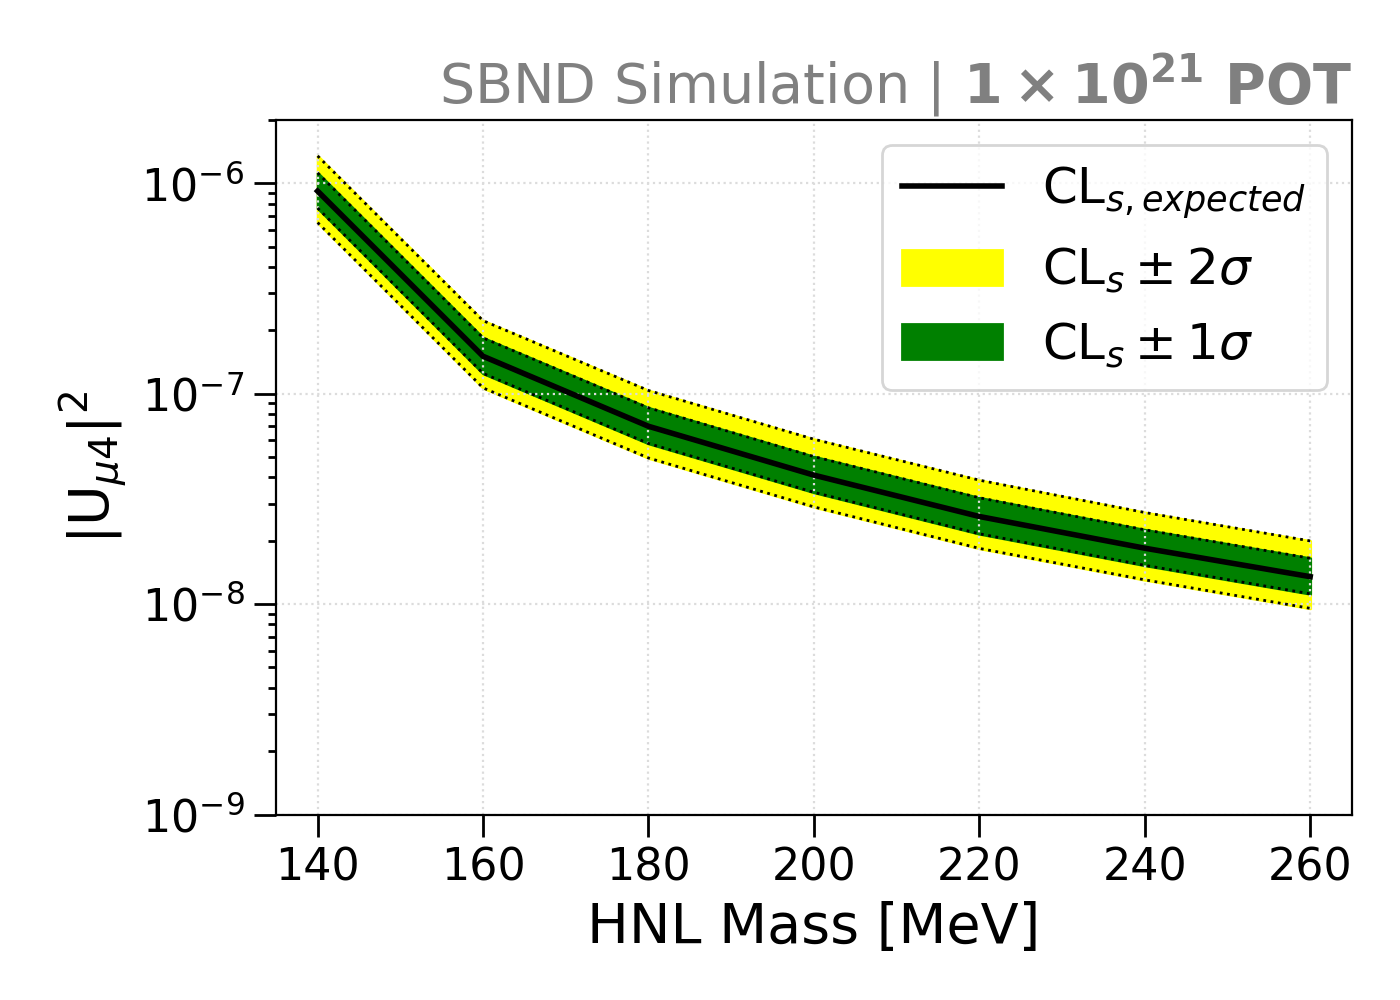
\includegraphics[width=\textwidth]{sensitivity_loose}
            \caption{The lenient distribution}%
        \end{subfigure}
        \begin{subfigure}[b]{0.495\textwidth}
            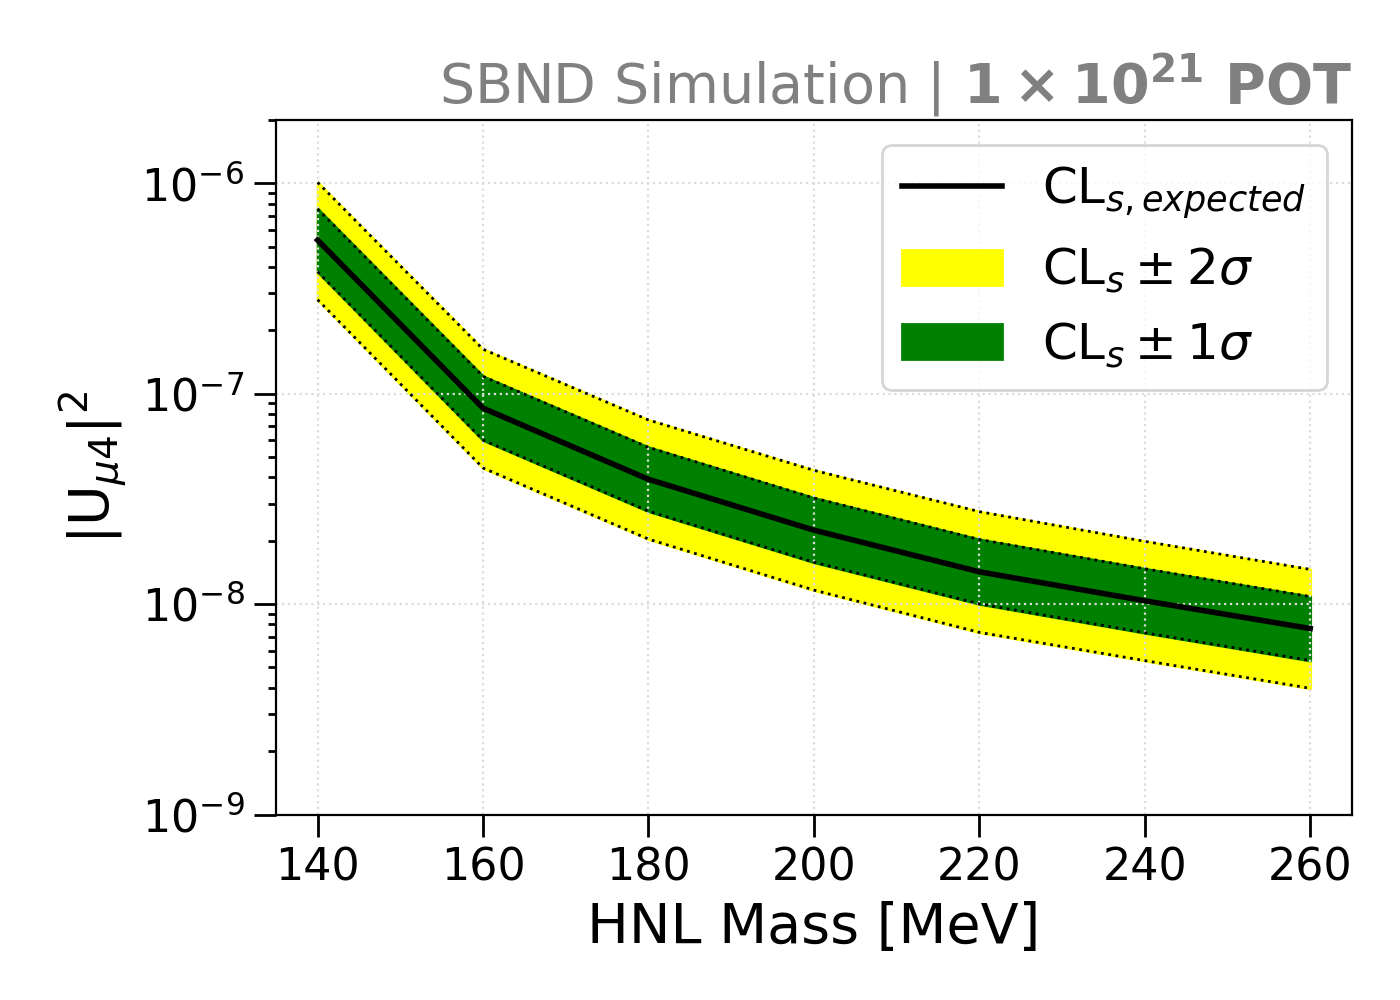
\includegraphics[width=\textwidth]{sensitivity_strict}
            \caption{The stringent distribution}%
        \end{subfigure}
    \caption[Expected Limits on the Coupling $|U_{\mu4}|^2$ for Majorana HNLs]{
    Expected limits and the Brazil bands on the coupling $|U_{\mu4}|^2$ for Majorana HNLs from (a) the lenient and (b) stringent arrival time distribution.
    }
    \label{fig:nupi0_reco_result}
\end{figure}

However, the width of the Brazil band of the stringent result is larger than the lenient result, indicating that the stringent result has larger uncertainties.
This is likely due to the limited statistics of the background MC samples after the stringent selection.
As can be observed from bins at the edge of the arrival time distribution shown in Fig. \ref{fig:final_strict}, the limited background statistics might be insufficient to describe the underlying distribution, which can lead to large statistical fluctuations.                                  
Although the stringent distribution leads to a more competitive result, a future iteration of this selection is recommended to perform on larger statistics MC samples so that the statistical uncertainty can be better constrained.

Fig. \ref{fig:nupi0_reco_full_edge} shows the comparison between limits setting using the entire distribution and only the first and last 4 bins, which are referred to as the timing cut (See Section \ref{sec:select_result}). 
The expected limits are the same for both cases.
The result demonstrates that the first and last 4 bins are the highest signal-to-background ratio bins of the entire distribution, and therefore are the main contributor to the limits.
This provides a useful insight for future iterations of this analysis indicating the region on the arrival time distribution should be focused on when performing the selection.
A recommendation is to focus on optimising the signal-to-background only in the edge region.
Another recommendation is to develop different selections for different regions of the arrival time distribution, capitalising on their different signal-to-background ratios.

\begin{figure}[htb!]
        \begin{subfigure}[b]{0.495\textwidth}
            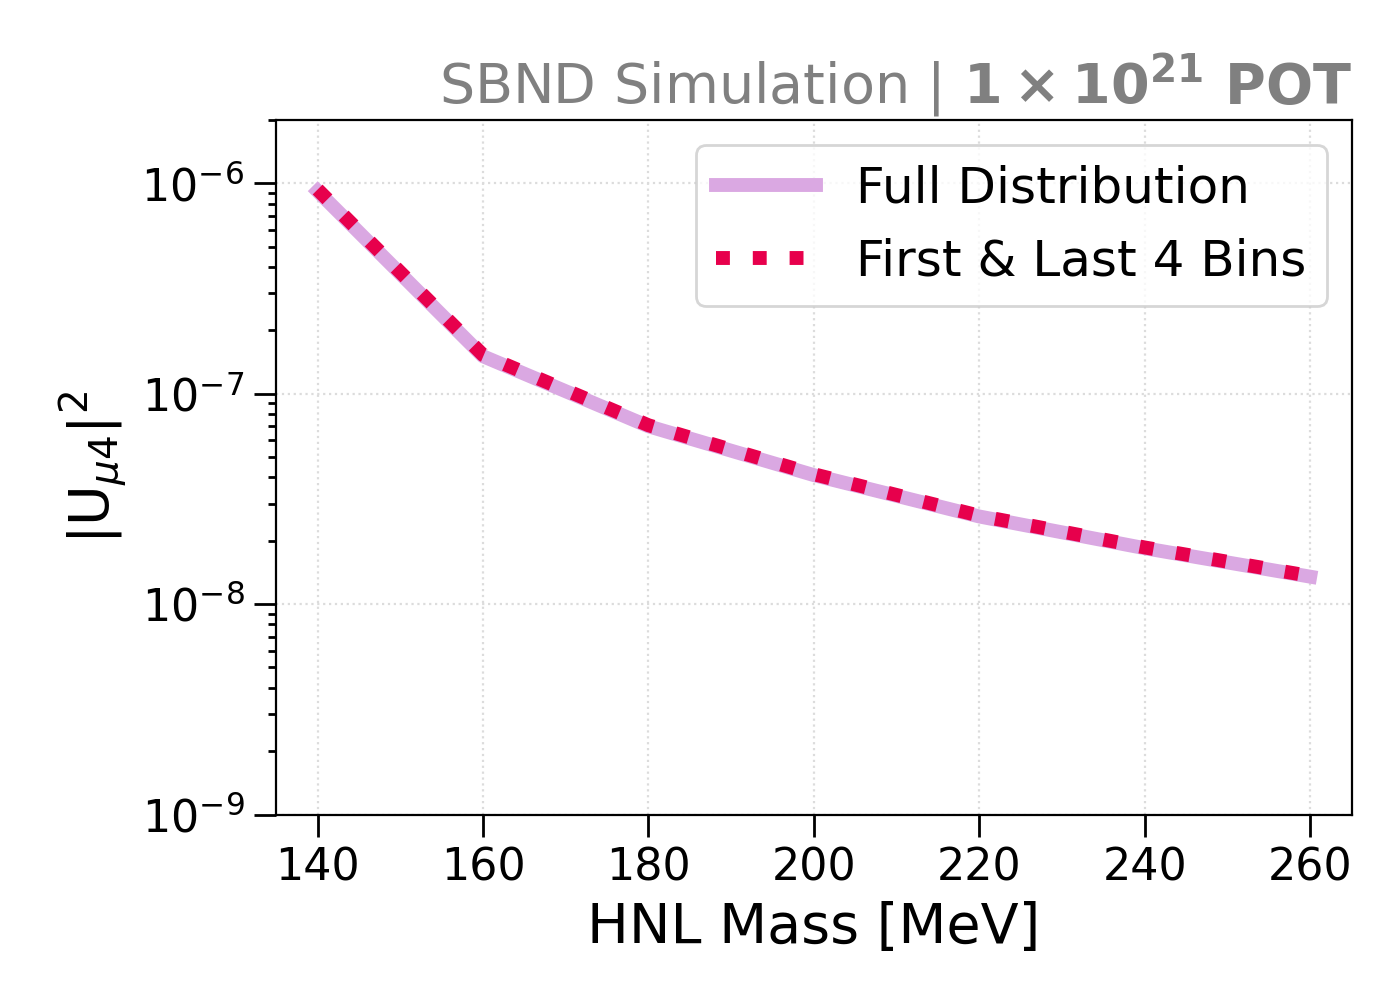
\includegraphics[width=\textwidth]{sensitivity_loose_full_edge}
            \caption{The lenient distribution}%
        \end{subfigure}
        \begin{subfigure}[b]{0.495\textwidth}
            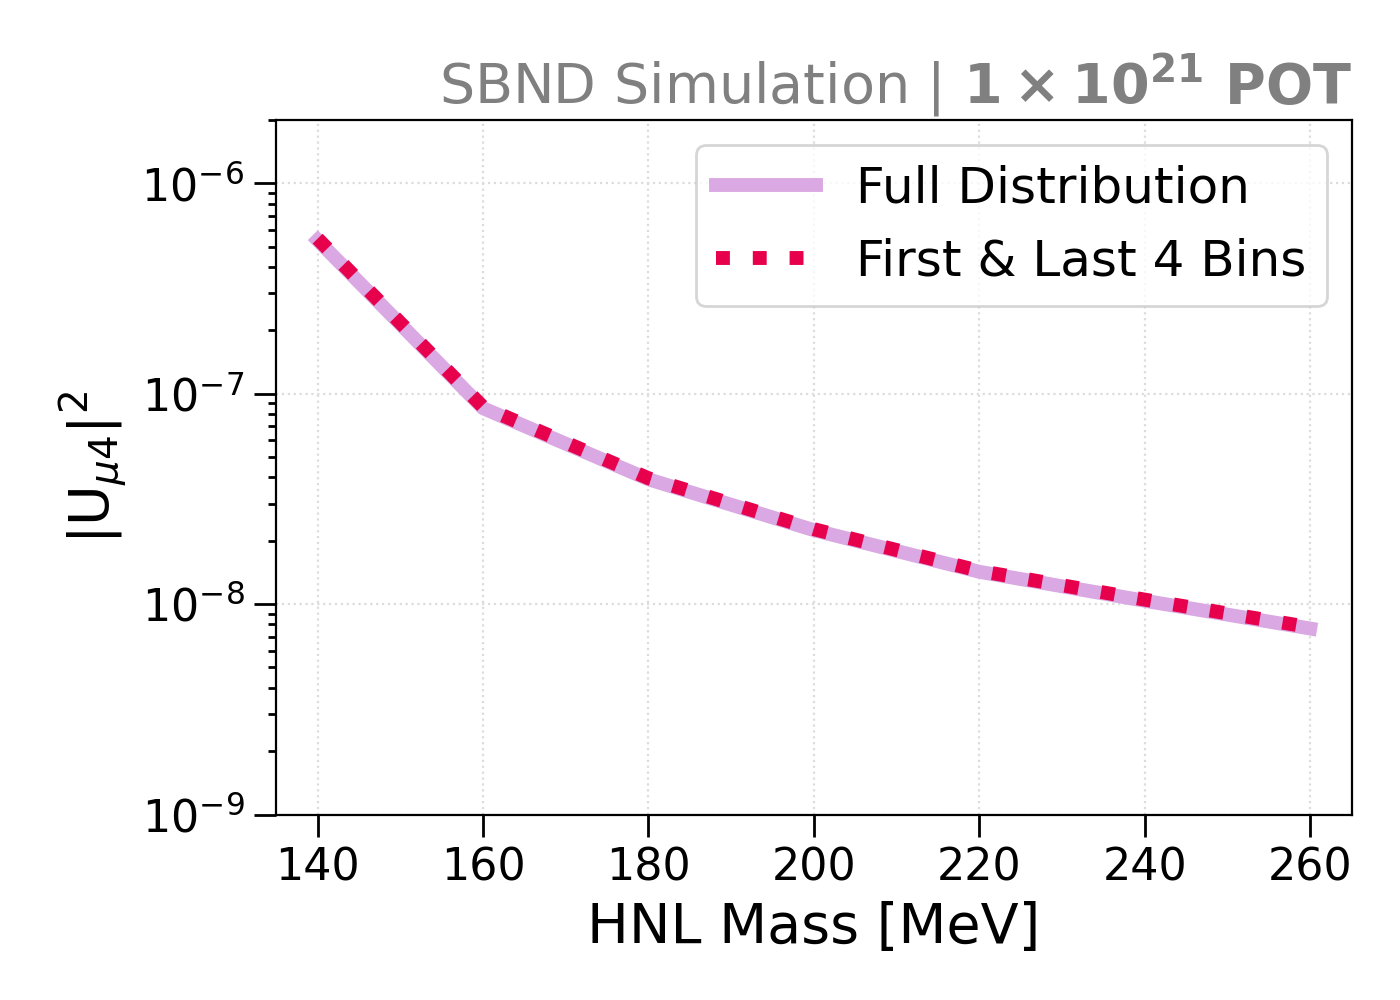
\includegraphics[width=\textwidth]{sensitivity_strict_full_edge}
            \caption{The stringent distribution}%
        \end{subfigure}
    \caption[Comparison Between Limits Setting using the Entire Distibution and Only Edge Bins]{Comparison between limits setting using the entire distribution and only the edge bins of (a) the lenient and (b) stringent arrival time distribution.}
    \label{fig:nupi0_reco_full_edge}
\end{figure}

Fig. \ref{fig:nupi0_reco_truth} shows the upper limits from all three arrival time distributions.
The result from the smeared true distribution, as shown by the green line, is significantly more competitive than the results using reconstructed distributions, as shown by the red and blue lines.
Limits from the smeared true distribution range from the level of $1.81 \times 10^{-7}$ to $2.46 \times 10^{-9}$ across the mass range of 140 - 260 MeV. 
As detailed in Section \ref{sec:truth_bucket}, the smeared true distribution was produced under the assumption of an improved timing resolution to explore its impact on sensitivity. 
The smeared true arrival time distribution of backgrounds has a Gaussian width of 1.73 ns as compared to $1.99$ ns of the lenient/stringent distribution.
The impact of the timing resolution improvement is evident in Fig. \ref{fig:final_truth}, where the background rate is lower and the signal rate is significantly higher for edge bins of the smeared true distribution.
The exceptionally high signal-to-background ratios of the edge bins therefore drives the limits more aggressively. 
%resulting in a higher signal-to-noise ratio

\begin{figure}[ht!]
    \centering
    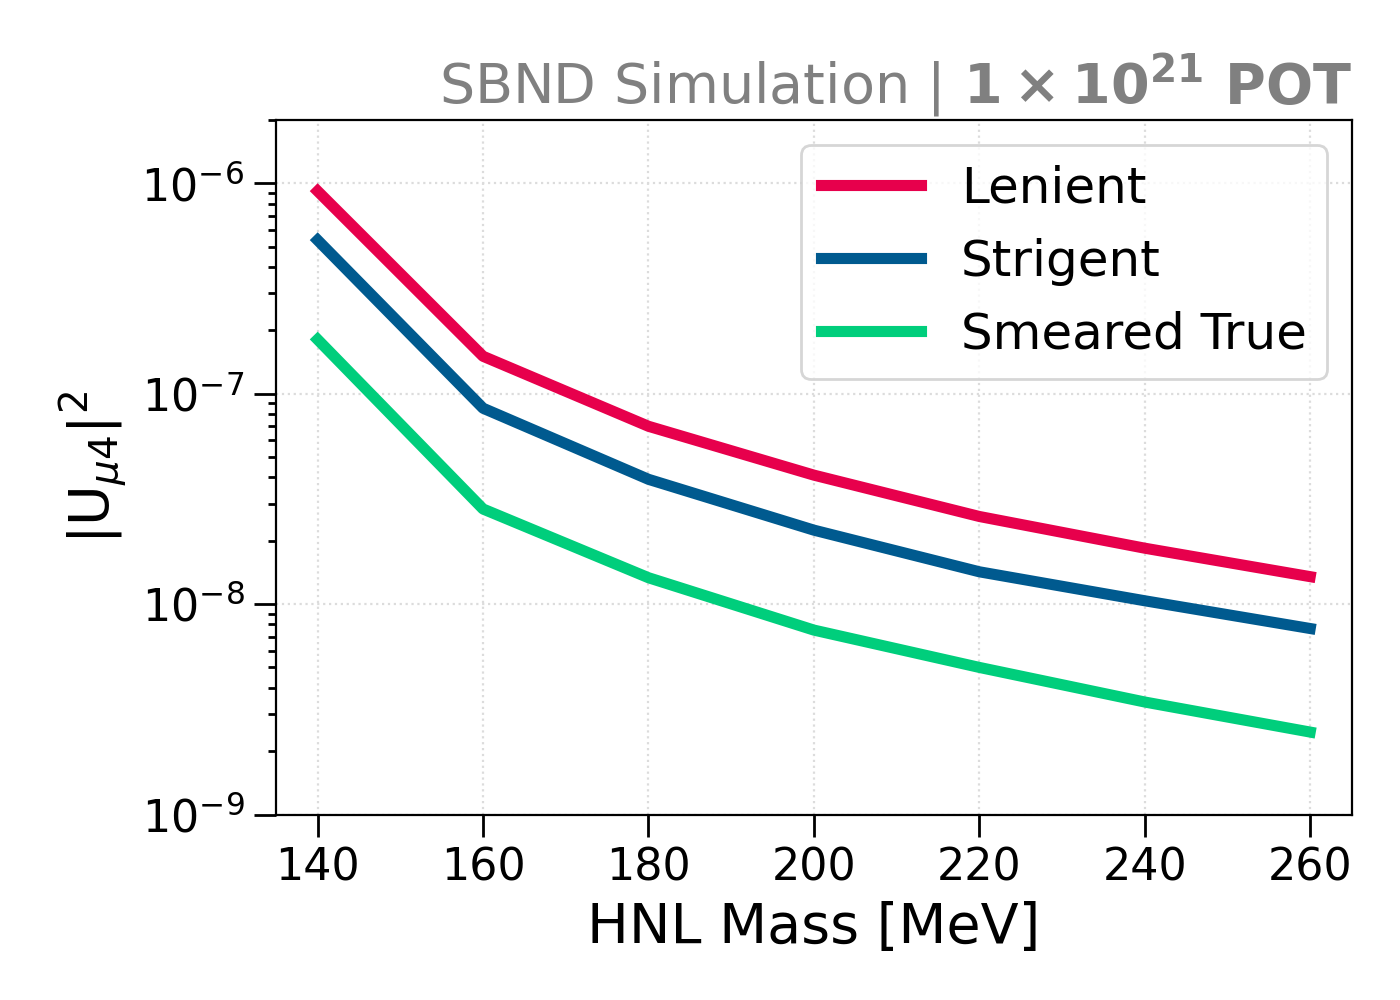
\includegraphics[width=0.65\textwidth]{sensitivity_strict_loose_truth}
    \caption[Comparison Between Limits Setting using the Lenient, Stringent and Smeared True Distribution]{Comparison between limits resulting from the lenient and stringent reconstructed distributions and the smeared true arrival time distribution.}
    \label{fig:nupi0_reco_truth}
\end{figure}

This presents a positive outlook as an area for improvement for SBND to achieve more competitive results in the search for HNLs.
Particularly, this can be done with a more sophisticated timing reconstruction that can resolve the beam bucket with higher resolution $< 2$ ns.
The expected upper limits at the 90\% C.L. and the Brazil bands acquired from the three arrival time distributions are summarised below in Table \ref{table:result}.  

\begin{table}[htbp!]
	\caption[Summary of Expected Limits on the Coupling $|U_{\mu4}|^2$ of Majorana HNLs]{Summary of expected limits on the coupling $|U_{\mu4}|^2$ of Majorana HNLs at the C.L. of 90\% predicted for SBND.}
\label{table:result}
\begin{center}
	\begin{tabular}{|c| c | c | c | c | c | c|} 
\hline 
& \textbf{Mass [MeV]} & \textbf{Expected Limit} & \textbf{+1$\sigma$} & \textbf{-1$\sigma$} & \textbf{+2$\sigma$} & \textbf{-2$\sigma$}\\

\hline &&&&&& \\[-1.5ex]
\multirow{6}{*}{\rotatebox[origin=c]{90}{\parbox[c]{3.65cm}{\centering \textbf{Lenient} }}} 

& 140 & $9.18\times10^{-7}$ & $1.12\times10^{-6}$ & $7.62\times10^{-7}$ & $1.35\times10^{-6}$ & $6.51\times10^{-7}$ \\
& 160 & $1.51\times10^{-7}$ & $1.84\times10^{-7}$ & $1.25\times10^{-7}$ & $2.22\times10^{-7}$ & $1.07\times10^{-7}$ \\
& 180 & $7.00\times10^{-8}$ & $8.57\times10^{-8}$ & $5.80\times10^{-8}$ & $1.04\times10^{-7}$ & $4.95\times10^{-8}$ \\
& 200 & $4.10\times10^{-8}$ & $5.02\times10^{-8}$ & $3.40\times10^{-8}$ & $6.08\times10^{-8}$ & $2.90\times10^{-8}$ \\
& 220 & $2.61\times10^{-8}$ & $3.20\times10^{-8}$ & $2.16\times10^{-8}$ & $3.88\times10^{-8}$ & $1.84\times10^{-8}$ \\
& 240 & $1.84\times10^{-8}$ & $2.26\times10^{-8}$ & $1.53\times10^{-8}$ & $2.73\times10^{-8}$ & $1.30\times10^{-8}$ \\
& 260 & $1.35\times10^{-8}$ & $1.65\times10^{-8}$ & $1.12\times10^{-8}$ & $2.00\times10^{-8}$ & $9.55\times10^{-9}$ \\ [0.5ex]
\hline &&&&&& \\[-1.5ex]
\multirow{6}{*}{\rotatebox[origin=c]{90}{\parbox[c]{3.65cm}{\centering \textbf{Stringent} }}} 

& 140 & $5.37\times10^{-7}$ & $7.56\times10^{-7}$ & $3.80\times10^{-7}$ & $1.01\times10^{-6}$ & $2.80\times10^{-7}$ \\
& 160 & $8.53\times10^{-8}$ & $1.21\times10^{-7}$ & $6.02\times10^{-8}$ & $1.63\times10^{-7}$ & $4.43\times10^{-8}$ \\
& 180 & $3.92\times10^{-8}$ & $5.56\times10^{-8}$ & $2.76\times10^{-8}$ & $7.50\times10^{-8}$ & $2.04\times10^{-8}$ \\
& 200 & $2.25\times10^{-8}$ & $3.20\times10^{-8}$ & $1.58\times10^{-8}$ & $4.32\times10^{-8}$ & $1.17\times10^{-8}$ \\
& 220 & $1.42\times10^{-8}$ & $2.03\times10^{-8}$ & $1.00\times10^{-8}$ & $2.75\times10^{-8}$ & $7.34\times10^{-9}$ \\
& 240 & $1.04\times10^{-8}$ & $1.47\times10^{-8}$ & $7.31\times10^{-9}$ & $1.99\times10^{-8}$ & $5.39\times10^{-9}$ \\
& 260 & $7.65\times10^{-9}$ & $1.09\times10^{-8}$ & $5.39\times10^{-9}$ & $1.46\times10^{-8}$ & $3.98\times10^{-9}$ \\ [0.5ex]
\hline &&&&&& \\[-1.5ex]
\multirow{6}{*}{\rotatebox[origin=c]{90}{\parbox[c]{3.65cm}{\centering \textbf{Smeared True} }}} 

& 140 & $1.81\times10^{-7}$ & $2.45\times10^{-7}$ & $1.35\times10^{-7}$ & $3.21\times10^{-7}$ & $1.05\times10^{-7}$ \\
& 160 & $2.83\times10^{-8}$ & $3.84\times10^{-8}$ & $2.11\times10^{-8}$ & $5.05\times10^{-8}$ & $1.63\times10^{-8}$ \\
& 180 & $1.33\times10^{-8}$ & $1.81\times10^{-8}$ & $9.94\times10^{-9}$ & $2.38\times10^{-8}$ & $7.70\times10^{-9}$ \\
& 200 & $7.52\times10^{-9}$ & $1.02\times10^{-8}$ & $5.62\times10^{-9}$ & $1.34\times10^{-8}$ & $4.38\times10^{-9}$ \\
& 220 & $5.00\times10^{-9}$ & $6.78\times10^{-9}$ & $3.73\times10^{-9}$ & $8.90\times10^{-9}$ & $2.90\times10^{-9}$ \\
& 240 & $3.42\times10^{-9}$ & $4.65\times10^{-9}$ & $2.55\times10^{-9}$ & $6.10\times10^{-9}$ & $1.99\times10^{-9}$ \\
& 260 & $2.46\times10^{-9}$ & $3.34\times10^{-9}$ & $1.84\times10^{-9}$ & $4.39\times10^{-9}$ & $1.44\times10^{-9}$ \\ [0.5ex]
\hline
\end{tabular}
\end{center}
\end{table}

\subsection{Comparison With Other Experiments}

Fig. \ref{fig:sensitivity} shows the expected upper limits of SBND on the coupling $|U_{\mu4}|^2$ of Majorana HNLs, comparing against existing experimental results as previously discussed in Section \ref{sec2Previous}.
All limits presented here are at the 90\% C.L.

For the limits acquired from the lenient and stringent distributions, as shown by the solid red and blue line respectively, they are comparable to existing limits.
The lenient limit is almost the same as the limit achieved by the MicroBooNE experiment \cite{uboone1, uboone2, uboone3}, as shown by the solid light blue line.
On the other hand, the stringent limit is slightly more competitive than MicroBooNe, excluding a new region of the coupling in the mass range $< 200$ MeV.
However, in the mass range $> 200$ MeV, the phase space is already excluded by the E949 \cite{E949} and NA62 experiments \cite{NA62A, NA62B}, as shown by the dashed pink and orange lines.
These two limits feature the first benchmark of SBND in the HNL regime as compared to other experiments, given the current detector and reconstruction capabilities.

The limits acquired from the smeared true distribution, as shown by the green line, is the most competitive out of the three limits presented here.
The limits are projected to exclude a new region beyond the existing limits from the MicroBooNE, E949 and NA62 experiments.
This demonstrates the potential of the physics capability of SBND, under the assumption of an exposure of $1 \times 10^{21}$ POT and an exceptional timing reconstruction with a resolution of 1.73 ns.
The POT exposure presented here is equivalent to 3 years of physics data taking, which allows for a lot of time and opportunities to work on improving the timing reconstruction of SBND to achieve the target resolution from the time of writing.
In comparison to the future DUNE experiment \cite{HNLSilvia}, DUNE is projected to have statistics to set upper limits surpassing SBND and nearly all existing limits in this mass range.

\begin{figure}[b!]
    \centering
    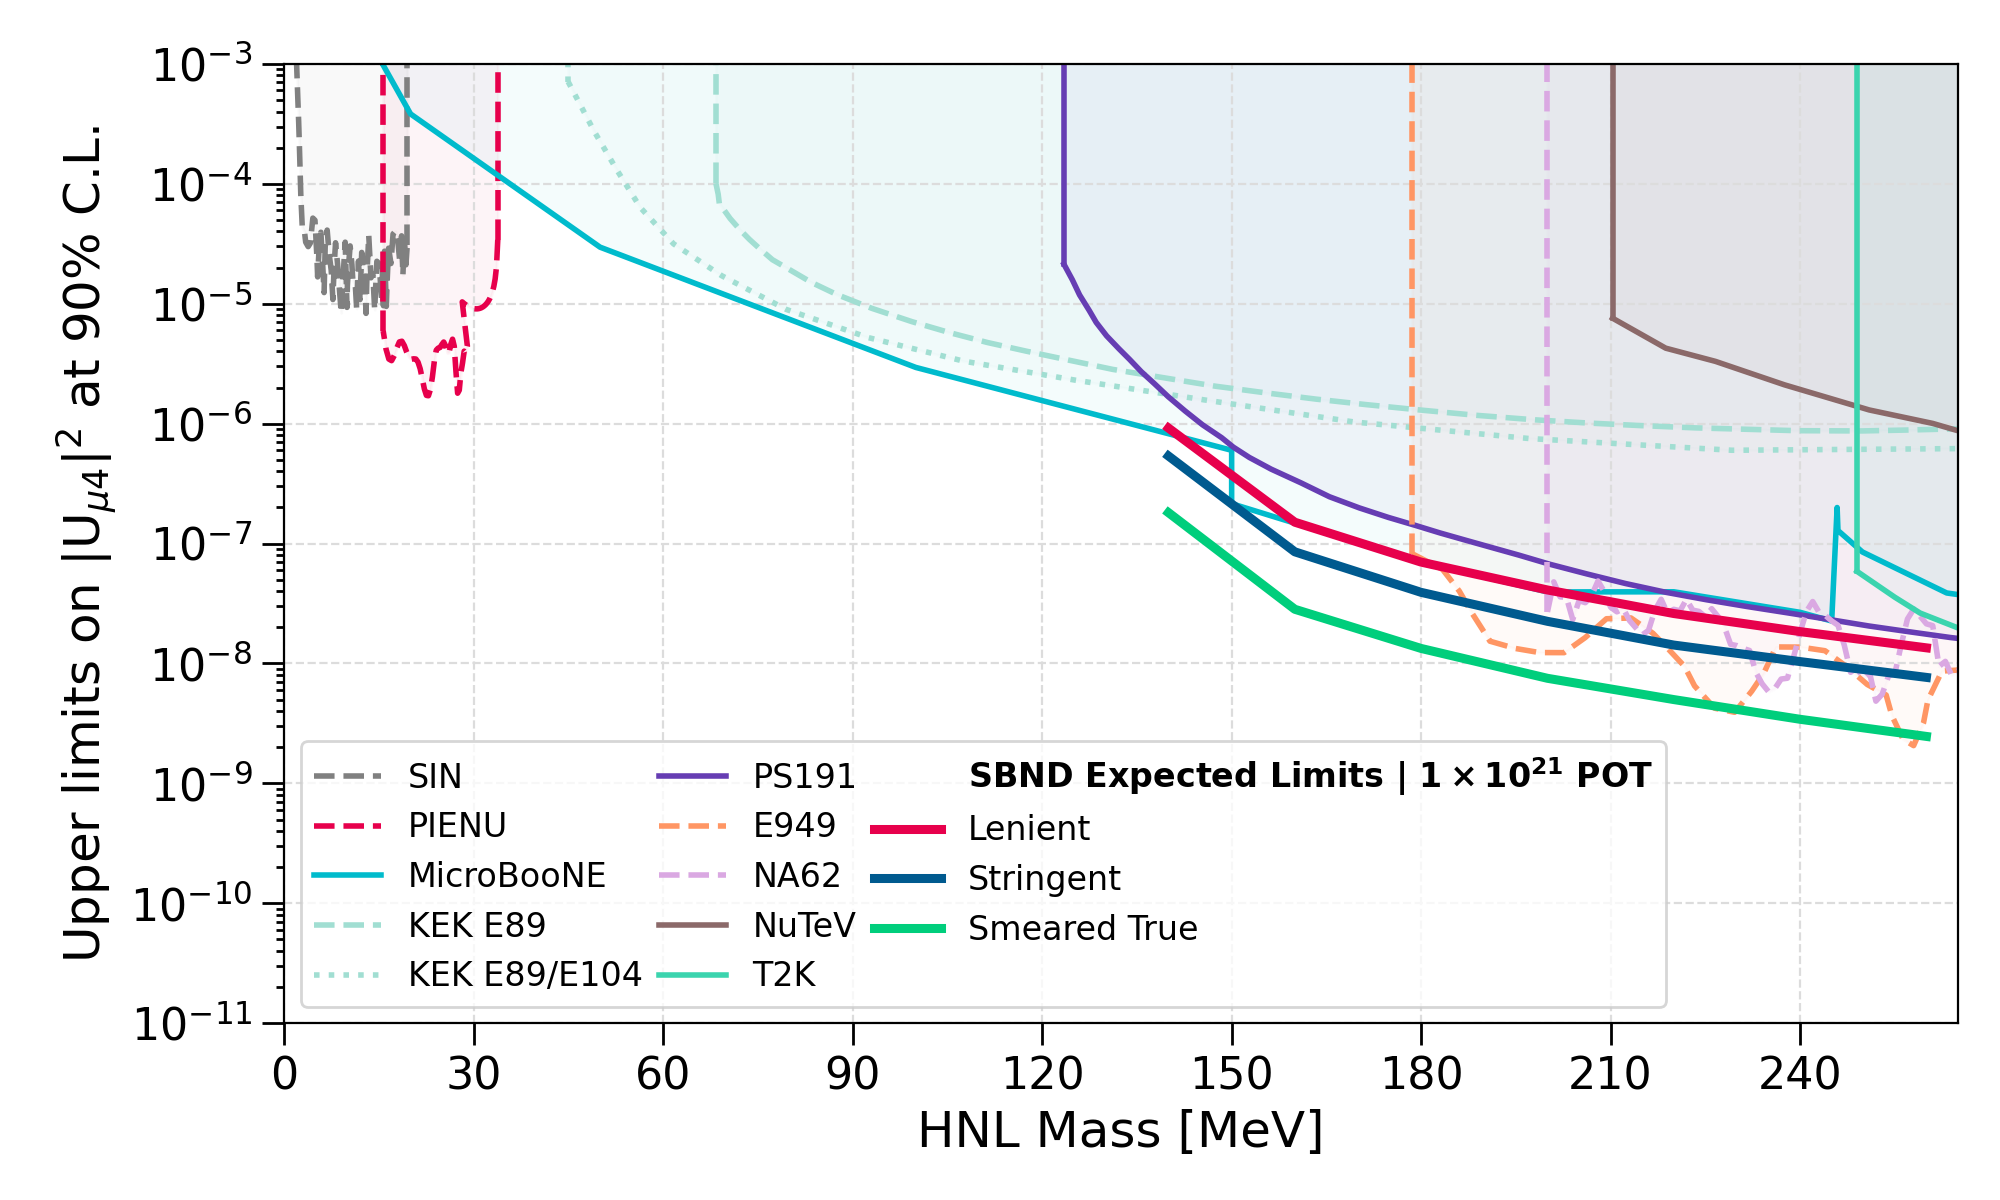
\includegraphics[width=\textwidth]{sensitivity}
    \caption[Comparison Between SBND Expected Limits and Existing Limits]{
Upper limits on the coupling $|U_{\mu4}|^{2}$ at the 90\% confidence level for Majorana HNLs in the mass range of $0 < m_{N} < 265$ MeV.
SBND expected limits are compared with existing experimental results, including SIN \cite{SIN3}, PIENU \cite{PIENU}, MicroBooNE \cite{uboone1, uboone2, uboone3}, KEK E89 \cite{KEK2}, KEK E89/E104 \cite{KEK3}, PS191 \cite{PS191C}, E949 \cite{E949}, NA62 \cite{NA62B}, NuTeV \cite{NuTeV}, T2K \cite{t2k} and expected results from DUNE \cite{HNLSilvia}.
}
\label{fig:sensitivity}
\end{figure}

%********************************** %First Section  **************************************
\section{Concluding Remarks}
\label{sec:result_remarks}

Three expected upper limits on the coupling $|U_{\mu4}|^2$ of Majorana HNLs are presented in this chapter to demonstrate the range of the physics capability of SBND.
The limits from the lenient and stringent arrival time distribution demonstrate the current performance of SBND, which is currently comparable to existing experimental limits.
The limits from the smeared true distribution are the most competitive that can probe region not yet explored by other experiments.
These limits also demonstrate the potential that SBND can achieve if the timing reconstruction is improved with a better resolution.

The first iteration of this analysis provides some guidelines applicable to future work in the next couple of years to further the search for HNLs at SBND.
Detector systematics should be included in uncertainty propagation, with parameters that are impactful to physics measurements identified when SBND is operational.
Secondly, due to the aggressive background rejection, the analysis should be performed on larger background MC samples, $\mathcal{O}$(10$^6$ events) compared to the present $\mathcal{O}$(10$^5$ events), to avoid statistical fluctuations.
Moreover, improving the shower reconstructions will enable better identification of the boosted features of HNL showers, including high energy profiles and forward-going angles.
Finally, developing a more sophisticated method incorporating the extra timing information of beam arrival and trigger signals can further improve the resolution of the timing reconstruction.
These improvements will benefit not only the HNL analysis but any other analysis that exploits the Gaussian tails of the beam bucket to either look for a new signal or reject cosmic backgrounds.

%Although ambitious, this goal is within reach in the next couple of years given the ongoing work towards a nanosecond timing resolution at SBND, one of which was presented in Chapter \ref{ChapterDAQ} and many more to be expected in the near future.
%Finally, the results of the smeared true distribution also motivate the need for a resolution improvement when reconstructing the arrival time distribution.
%The preparation work towards the nanosecond resolution has already begun with the DAQ readout electronics and the implementation of the SPEC-TDC for high precision timestamping.  
